%% LyX 1.3 created this file.  For more info, see http://www.lyx.org/.
%% Do not edit unless you really know what you are doing.
\documentclass[brazil,ruledheader]{abnt}
\usepackage[T1]{fontenc}
\usepackage[latin1]{inputenc}
%\usepackage[vlined,boxruled,linesnumbered,portuguese]{algorithm2e}
\usepackage[ruled,longend,lined,linesnumbered,portuguese]{algorithm2e}
% Escrita dos algoritmos
\usepackage{amssymb,amsmath}
%\usepackage[dvipdf]{graphicx,color}
\usepackage{graphicx,color}
\usepackage{lscape}



\makeatletter
\usepackage{babel}
\makeatother
\begin{document}

\autor{Walace de Souza Rocha}


\titulo{Algoritmo GRASP para o Problema de Tabela-horário de Universidades}


\orientador{Maria Claudia Silva Boeres}


\coorientador{Maria Cristina Rangel}


\comentario{Dissertação apresentada como requisito parcial para obtenção do Grau de Mestre em Ciência
da Computação pela Universidade Federal do Espírito Santo.}


\instituicao{Departamento de Informática \par Centro Tecnológico\par Universidade
Federal do Espírito Santo}


\local{Vitória - ES, Brasil}


\data{28 de Fevereiro de 2013}

\capa

\folhaderosto

\begin{folhadeaprovacao}
Dissertação apresentada como requisito parcial para obtenção do Grau de Mestre em Ciência da Computação sob o título \textit{``\ABNTtitulodata''},
defendida por \ABNTautordata~e aprovada em \ABNTdatadata, em Vitória,
Estado do Espírito Santo, pela banca examinadora constituída pelos
professores: \setlength{\ABNTsignthickness}{0.4pt}

\assinatura{Profª Drª Maria Claudia Silva Boeres\\Universidade Federal do Espírito Santo\\ Orientadora}
\assinatura{Profª Drª Maria Cristina Rangel\\Universidade Federal do Espírito Santo\\ Co-orientadora}
\assinatura{Prof. Dr. Flávio Miguel Varejão\\ Universidade Federal do Espírito Santo}
\assinatura{Prof. Dr. Haroldo Gambini Santos\\ Universidade Federal de Ouro Preto}
\end{folhadeaprovacao}

\begin{resumo}
O problema de tabela-horário é de grande destaque na área de otimização combinatória. Dado um conjunto de disciplinas, alunos, professores e salas, o problema consiste em alocar aulas em um número limitado de horários e salas, respeitando algumas restrições. As formulações são variadas, o que às vezes dificulta a comparação de trabalhos. Apesar das diferenças, ele é classificado em três classes principais: tabela-horário de exames, de escolas e de universidades. Este trabalho trata especificamente de tabela-horário de universidades e é adotada a formulação três do campeonato internacional de tabela-horário ITC-2007. O problema é resolvido com a meta-heurística GRASP. {\it Hill Climbing} e {\it Simulated Annealing} são usados como fase de busca local do algoritmo e {\it Path-relinking} é implementado para melhorar a versão básica. Testes foram feitos simulando as mesmas regras do campeonato e os resultados obtidos estão competitivos com os obtidos pelos finalistas do ITC-2007.
\end{resumo}

\begin{abstract}

The timetabling problem is of great interest in the combinatorial optimization field. Given a set of disciplines, students, teachers and classrooms, the problem consists in to allocate lectures in a limited number of timeslots and rooms, respecting some restrictions. The formulations are varied, which sometimes makes it difficult to compare to other studies. Despite the differences, it is classified into three main classes: exams timetabling, schools timetabling and universities timetabling. This work specifically treats the universities timetabling and is adopted the third formulation of international timetabling competition - ITC-2007. The problem is solved with the GRASP metaheuristic. Hill Climbing and Simulated Annealing are used as local search phase of the algorithm and Path-relinking is implemented to improve the basic version. Tests were carried out simulating the same competition rules and the results are competitive with those obtained by the ITC-2007 finalists.
\end{abstract}

\chapter*{Dedicatória}

Dedico este trabalho a todos familiares, amigos e professores que contribuiram de alguma forma para que sua conclusão fosse possível.

\chapter*{Agradecimentos}

Agradeço primeiramente a Deus pela capacidade física e intelectual para realização deste trabalho.

À minha esposa Iris por estar sempre ao meu lado me incentivando.

Também agradeço às professoras Claudia e Cristina pelos ensinamentos nesta jornada e por tornarem o desenvolvimento da pesquisa mais agradável. Aos demais professores do Departamento de Informática pela importância na minha formação acadêmica.

%À direção do Núcleo de Processamento de Dados da UFES pelo apoio necessário

À CAPES pelo apoio financeiro.

\tableofcontents{}\listoffigures



\listoftables

\listofalgorithms


\chapter{Introdução\label{cap:introducao}}

%\vfill{}
%\vfill{}

%Neste capítulo são apresentados o objetivo desta dissertação e a estrutura da mesma.
%\newpage

%\section{Apresentação do problema}

Os problemas de \textit{scheduling} tratam a alocação de recursos em determinados horários satisfazendo algumas restrições. Os problemas de tabela-horário são um subconjunto importante desta área e as aplicações são variadas como, por exemplo, elaboração de escala de funcionários e agendamento de partidas para campeonatos esportivos.

No caso específico de tabela-horário de escolas, o problema consiste em alocar um conjunto de aulas em um número pré-determinado de horários, satisfazendo diversas restrições envolvendo professores, alunos e o espaço físico disponível. A solução manual deste problema não é uma tarefa trivial e as instituições de ensino precisam resolvê-lo anualmente ou semestralmente. Nem sempre a alocação manual é satisfatória, visto que é difícil contemplar todos os anseios das partes envolvidas. 

Por esta razão, atenção especial tem sido dada a solução automática de tabela-horário. Nos últimos cinquenta anos, começando com \cite{gotlieb62}, este problema ganhou grande destaque na área de otimização combinatória, tendo diversos trabalhos publicados \cite{Schaerf95asurvey,Lewis2007:survey}.

%\section{Motivação para o problema}

O problema de tabela-horário está entre os mais difíceis da área de otimização combinatória. Sua dificuldade aumenta à medida em que são adicionadas restrições. Em \cite{Schaerf95asurvey} pode ser visto que ele é classificado como NP-completo para a maioria das formulações. Assim, a solução exata só pode ser garantida para instâncias bem pequenas, que não correspondem às instâncias reais da maioria das instituições de ensino.

Existe uma necessidade de propor algoritmos cada vez mais eficientes que produzam soluções satisfatórias para o problema em um tempo viável, independente do tamanho da instância. Devido à complexidade do problema, métodos exaustivos são descartados. Por serem relativamente simples de implementar e produzirem bons resultados, diferentes meta-heurísticas tem sido aplicadas, com destaque para \textit{Simulated Annealing} \cite{CDGS11b}, Algoritmo Genético \cite{Erben95agenetic} e Busca Tabu \cite{elloumi2008}. Dentre as meta-heurísticas já aplicadas ao problema, existe um esforço para encontrar melhorias e conseguir melhores resultados.

Algumas meta-heurísticas ainda não foram aplicadas ao problema, mas tem se mostrado eficientes em outros problemas de otimização combinatória. Uma delas é o GRASP, que já foi aplicado no problema de satisfabilidade \cite{ResFeo96a}, conjunto independente máximo \cite{FeoResSmi94}, cobertura de conjuntos \cite{Pessoa2012}, entre outros, mas em se tratando de tabela-horário só há trabalhos publicados para o caso de escolas primárias e secundárias. Deseja-se investigar a sua eficiência no caso específico de universidades.

\section{Objetivos deste trabalho}

O objetivo principal deste trabalho é resolver o problema de tabela-horário de universidades usando a meta-heurística GRASP (\textit{Greedy Randomized Adaptive Search Procedures}). Pelo fato de existirem diversas formulações para o problema, escolhemos a proposta no ITC-2007 (\textit{International Timetabling Competition - 2007}) \cite{itc2007}  pois tem sido bastante utilizada na área. A razão principal desta escolha é facilitar a comparação dos resultados com outros algoritmos propostos na literatura.

Para atingir este objetivo foi necessário estudar a formulação do ITC-2007 e propor uma implementação eficiente dos dados. Além de aplicar o GRASP com construção de uma solução inicial e refinamento com busca local, será implementada mais uma etapa de melhoramento com a técnica \textit{Path-Relinking}. Todas estas etapas do algoritmo serão detalhadas na seção \ref{sec:estrutura_grasp}.

O ITC-2007 estimulou um maior debate entre a comunidade que pesquisa tabela-horário e muitas técnicas de resolução tem sido desenvolvidas e/ou aprimoradas graças a este campeonato. Outra grande contribuição é a disponibilização de instâncias bem próximas à realidade das universidades.

Vale ressaltar que o ITC-2007 dividiu o campeonato em três formulações, sendo que os competidores podiam concorrer independentemente em cada uma delas. Cada formulação específica tem seu próprio conjunto de instâncias. A primeira formulação é específica para aplicação de exames finais. A segunda  e terceira formulação tratam a alocação semanal das aulas de uma universidade. A diferença básica é que a segunda formulação, chamada de \textit{post enrolment} (pós matrícula) trata o problema considerando os dados de matrícula dos alunos, enquanto que na terceira as informações levam em conta os currículos que compõem a universidade. Currículos são definidos como grupos de disciplinas que têm alunos em comum e não devem ser alocadas no mesmo horário.

Na terceira formulação os conflitos de horários entre as disciplinas são estabelecidos pela composição dos currículos, logo, disciplinas do mesmo currículo não podem ser alocadas no mesmo horário. Por outro lado, na segunda formulação os conflitos são estabelecidos pelas matrículas dos alunos. Desta forma, aulas de disciplinas que um mesmo aluno matriculou não podem ser alocadas no mesmo horário.

Adotamos neste trabalho a terceira formulação por ser considerada, dentre as três, a mais próxima do que acontece na prática nas universidades brasileiras. Esta formulação será explicada em detalhes no capítulo \ref{cap:proposta-trabalho}.

Durante o desenvolvimento da pesquisa foi lançada a terceira edição do campeonato, o ITC-2011. Esta edição trouxe uma formulação mais voltada para escolas, conhecida internacionalmente como \textit{high school}. Como um dos nossos objetivos iniciais era resolver o problema para universidades, decidimos continuar trabalhando com o ITC-2007.


\section{Organização do texto}

No capítulo \ref{cap:estado-da-arte} é apresentada uma revisão bibliográfica listando as principais técnicas de solução do problema. No capítulo \ref{cap:proposta-trabalho} é apresentada a formulação do problema segundo o ITC-2007. O algoritmo GRASP e sua aplicação no problema são descritos no capítulo \ref{cap:grasp}. No capítulo \ref{cap:resultados} são apresentados detalhes de implementação, instâncias de testes e os resultados obtidos. No capítulo \ref{cap:conclusao} são listadas as conclusões obtidas no trabalho e enumerados alguns trabalhos futuros.


\chapter{Revisão Bibliográfica\label{cap:estado-da-arte}}

%\vfill{}
%\begin{flushright}{}``\emph{Navegar é preciso, viver não.}''\\
%{\small Luís de Camões}\end{flushright}{\small \par}
%\vfill{}

%Neste capítulo são apresentados alguns conceitos básicos e uma revisão bibliográfica.
%\newpage

%\section{Introdução}

O problema de tabela-horário (\textit{Timetabling}) deriva do problema de escalonamento (\textit{scheduling}) e foi definido por \cite{wren} como a alocação, submetida a restrições, de determinados recursos a eventos colocados em um número limitado de períodos de tempo e locais, de forma a satisfazer tanto quanto possível um conjunto de objetivos estabelecidos.

O problema de tabela-horário pode ser aplicado a diversos tipos de situações, entre os quais inclui-se:

\begin{itemize}

\item Escalas de Trabalhadores (\textit{Employee Timetabling}): trata da alocação de
trabalhadores de uma empresa às suas tarefas em um conjunto de turnos de
trabalho dentro de um período fixo de tempo, geralmente semanal,
respeitando determinadas regras (restrições) pessoais e do trabalho. Em
\cite{nurse_rostering} e \cite{chiarandini} podem ser vistas abordagens deste problema;

\item Escalas de Condutores de Veículos de Transporte (\textit{Transportation Timetabling}):
Segundo \cite{laplagnetime} este problema determina a composição de um conjunto de turnos de condutores
de veículos para a operação de transporte diário, assegurando a cobertura
requerida e minimizando os custos operacionais;

\item Escalas de Jogos de Competições Esportivas (\textit{Sports Timetabling}): consiste na
programação de uma tabela de jogos de competições esportivas, satisfazendo
aos requisitos da competição e minimizando os custos, por exemplo, custo de viagens das equipes. \cite{nurmi2010framework, Ribeiro:2012:SBS:2340795.2340799} são exemplos deste tipo de abordagem;

\item Educacional (\textit{Educational Timetabling}): aborda a geração de tabela-horário para
instituições de ensino, que é o foco do estudo deste trabalho. Dos diversos
tipos de problemas de tabela-horário, o educacional é um
dos mais amplamente estudados. Este problema é analisado mais
detalhadamente a seguir.

\end{itemize}

O problema de tabela-horário não possui uma formulação única. Como pode ser visto em \cite{Schaerf95asurvey}, ao longo do tempo surgiram diversas modelagens. Essa variedade surgiu pelo fato das restrições do problema serem específicas a cada instituição de ensino.

Algumas coleções de instâncias, os \textit{benchmarks}, foram criadas. As disponíveis pelo campeonato ITC (versões 2002, 2007 e 2011) \cite{itc2007} são bastante utilizadas. Mas existem algumas outras, como o da Universidade de Toronto \cite{toronto_exames} e o da Universidade de Nottingham \cite{Burke96examinationtimetabling}, os dois para tabela-horário de exames.

Apesar das diferentes formulações, os problemas de tabela-horário possuem uma característica em comum: a separação das restrições em dois grupos, considerados como restrições fortes e fracas.

As restrições fortes são aquelas que não podem ser violadas. Elas restringem o conjunto de soluções para impedir certas situações irreais, como por exemplo, alunos assistindo mais de uma aula no mesmo horário ou uma sala sendo alocada para mais de uma aula no mesmo horário. Se uma tabela-horário não viola nenhuma restrição forte ela é dita ser uma solução viável.

As restrições fracas são aquelas que não interferem na viabilidade da solução, mas refletem certas preferências das instituições. É desejável, por exemplo, que um aluno não tenha aulas isoladas durante o dia ou que aulas da mesma disciplina sejam lecionadas na mesma sala. As restrições fracas podem possuir pesos diferentes para refletir sua importância na qualidade da solução.

O objetivo do problema é encontrar uma tabela-horário viável e que minimize a quantidade de violações fracas, portanto, um problema de minimização.

\section{Restrições abordadas no problema}

As restrições que são impostas ao problema de tabela-horário geralmente se referem a limitação do espaço físico e de horários, preferências de alunos e professores, além de certas exigências das instituições de ensino. As mais comuns nas diferentes formulações são:

\begin{itemize}
\item Professores não podem lecionar mais de uma aula no mesmo horário;
\item Alunos não podem assistir mais de uma aula no mesmo horário;
\item Todas as aulas da disciplina devem ser alocadas na semana;
\item A capacidade das salas deve ser adequada para os alunos matriculados;
\item As aulas não devem ser muito espalhadas durante o dia.
\end{itemize}

Algumas restrições são muito específicas e raramente aparecem na literatura. No trabalho de \cite{ConstantinoEtAl2010} a tabela-horário limita o deslocamento de alunos entre os prédios do campus da universidade.

Há certa variação na forma como uma mesma restrição é aplicada. Exemplo típico desta situação é a restrição de capacidade das salas. Em \cite{ConstantinoEtAl2010} as disciplinas não podem ser alocadas em salas cuja capacidade seja inferior a quantidade de alunos, portanto, uma restrição forte. Mas na terceira formulação do ITC-2007 essa mesma restrição é considerada fraca, ocorrendo uma penalização quando a quantidade de assentos é inferior a quantidade de alunos. Existem trabalhos, como em \cite{Shiau:2011:HPS:1860128.1860157}, que esta restrição não é nem considerada.

\section{Classificação do problema de tabela-horário educacional}

As diversas formulações do problema apresentadas na literatura variam devido à instituição envolvida (escola ou universidade) e também pelo conjunto de restrições que são abordadas. Contudo, todas as formulações podem ser classificadas em uma das três classes principais \cite{Schaerf95asurvey}:

\begin{itemize}

\item \textbf{Tabela-horário de Escola} Programação semanal para as turmas da escola, evitando que professores lecionem para duas turmas ao mesmo tempo ou que turmas assistam mais de uma aula no mesmo horário.

\item \textbf{Tabela-horário de Universidade} Programação semanal das aulas das disciplinas universitárias, minimizando a sobreposição de aulas que tenham alunos em comum.

\item \textbf{Tabela-horário de Exames} Programação para aplicação dos exames das disciplinas, evitando sobreposição de exames das disciplinas que tenham alunos em comum, procurando alocar os dias dos exames dos alunos com o maior intervalo possível. 

\end{itemize}

A tabela-horário de exames é usada somente nos finais de bimestre, trimestre ou semestre, enquanto as duas primeiras são soluções que devem ser usadas durante todo o período letivo. A diferença principal do problema no âmbito de escolas e universidades é que no segundo não há o conceito de turma, já que cada aluno escolhe o conjunto de disciplinas que irá cursar. Nas escolas (primárias e secundárias) todos alunos matriculados numa turma cursam as mesmas disciplinas.

\section{Abordagens de solução existentes\label{sec:abordagens}}

As técnicas usadas para resolver o problema de tabela-horário são bastante diversificadas. As mais antigas, as heurísticas construtivas \cite{Junginger:1986:TGS,papoulias}, foram baseadas no modo humano de resolver o problema: as aulas eram alocadas uma a uma até finalizar a construção da tabela. Conflitos eram resolvidos realizando trocas de aulas.

\cite{Neufeld} propuseram uma redução do problema ao problema de coloração de grafos. As aulas são representadas como vértices do grafo. Arestas conectam aulas que não podem ser alocadas no mesmo horário. A coloração do grafo resultante é então transformada na tabela-horário: cada cor representa um horário de aula. Propostas similares a esta foram aplicadas em \cite{deWerra85,Selim:1988}. Numa abordagem semelhante, \cite{Galinier20062547} propuseram o algoritmo \textit{Tabucol} (Busca Tabu para resolver coloração de grafos), que posteriormente também foi usado por \cite{geraldo_bello}.

\cite{deWerra82} reduziram o problema de tabela-horário ao problema de fluxo de redes. As aulas são representadas pelos vértices. Uma rede é criada para cada horário e o fluxo na rede identifica as aulas que são lecionadas no mesmo horário. Posteriormente, \cite{deWerra85} usou uma idéia similar, mas cada fluxo representa uma classe e os vértices são horários e professores. Outras abordagens com fluxo de redes foram usadas em \cite{dinkel1989or,chahal1989}.

Mais recentemente, as técnicas de solução para o problema têm recaído basicamente em três grupos: programação matemática, programação em lógica e, principalmente, meta-heurísticas.

Na área de programação matemática, bons resultados têm sido obtidos com programação inteira. Em \cite{lach_lubbecke} pode ser vista uma formulação completa do problema. Ela foi executada com CPLEX9 \cite{cplex} e conseguiu soluções com respostas bem próximas às melhores obtidas na competição ITC-2007. Em \cite{Burke_abranch-andcut} é usado um procedimento conhecido na programação linear como \textit{branch-and-cut}. O problema inicialmente é resolvido sem as restrições de integralidade. Em seguida são usados planos de corte para se obter uma resposta com valores inteiros. Com um tempo de execução aproximado de 15 minutos no CPLEX10, esse algoritmo conseguiu encontrar a solução ótima para duas instâncias da competição. Esses dois trabalhos citados são de grande importância pois são capazes de fornecer limites inferiores para as quantidades de violações das restrições fracas para cada instância do ITC-2007. Em \cite{ribeiro2006integer} pode ser vista uma modelagem em programação inteira mais específica para escolas brasileiras de ensino fundamental.

Alguns resultados relevantes também têm sido encontrados com programação em lógica. \cite{springerlink:10.1007/s10479-012-1081-x} apresentam uma formulação usando \textit{MaxSAT} que conseguiu melhorar quase metade das respostas até então conhecidas para as instâncias do ITC-2007. Os trabalhos de \cite{Gueret95buildinguniversity} e \cite{Goltz99universitytimetabling} adotam formulações diferentes do ITC-2007, mas destacam como programação em lógica combinada com programação por restrições podem implementar modelos bem flexíveis, em que restrições podem ser adicionadas, modificadas ou excluídas com pouca alteração de código-fonte.

Pode ser visto em \cite{Lewis2007:survey} que grande parte dos trabalhos recentes na área tem usado meta-heurísticas, tanto pela simplicidade quanto pelos bons resultados alcançados. Uma meta-heurística é um método heurístico para resolver de forma genérica problemas de otimização. Ela é genérica porque não se atém a detalhes específicos do problema que está sendo tratado, mas apenas especifica como o conjunto de soluções será explorado em busca da melhor solução. \textit{Simulated Annealing}, Algoritmo Genético e Busca Tabu são as mais utilizadas pelos pesquisadores mas há propostas com meta-heurísticas menos conhecidas, como a Busca de Harmonia \cite{albetar_harmony}.

Em \cite{Elmohamed98acomparison} foram investigadas diversas abordagens do \textit{Simulated Annealing}. Dentre as configurações possíveis, os melhores resultados foram obtidos com resfriamento adaptativo, reaquecimento e um algoritmo baseado em regras para gerar uma boa solução inicial. \cite{CDGS11b} usam \textit{Simulated Annealing} para resolver a segunda formulação do ITC-2007. Os autores conseguiram boas respostas para as instâncias, e em alguns casos, foram obtidas soluções melhores que as conhecidas no momento da comparação.

Algoritmos Genéticos também foram propostos para o problema, onde o cromossomo representa a tabela-horário e cada posição da tabela corresponde a um gene. Em seguida são definidas as operações genéticas de seleção, cruzamento e mutação, que visam gerar indivíduos cada vez melhores. Um indivíduo com bom valor \textit{fitness} representa uma tabela-horário bem avaliada de acordo com a função objetivo associada ao problema. \cite{Erben95agenetic} aplicaram esta técnica para tratar o problema de tabela-horário de universidades com muitas restrições, obtendo resultados promissores. Em \cite{Kanoh:2008:KGA} pode ser visto uma abordagem, também para universidades, em que se utiliza uma base de conhecimento para gerar a população inicial. Essa base de conhecimento é formada com informações de tabelas-horário de anos anteriores. \cite{massoodian2008} propuseram um algoritmo genético híbrido para resolver a terceira formulação do ITC-2007. O algoritmo foi considerado híbrido pois, além de aplicar os operadores genéticos, uma busca local foi utilizada nos melhores indivíduos ao final de cada geração.

Além das meta-heurísticas acima citadas, a Busca Tabu também tem sido aplicada com sucesso. Em \cite{elloumi2008} é apresentado um algoritmo para resolver o problema de tabela-horário de uma universidade tunisiana. \cite{Santos:2005:TSH} aplicaram a técnica no âmbito de escolas primárias de Minas Gerais e obtiveram respostas melhores que outros algoritmos propostos com Busca Tabu. Em \cite{Souza:2004:GSA} a Busca Tabu é aplicada como fase de busca local do GRASP, numa implementação também voltada para escolas.

As diversas restrições fortes e fracas fazem com que o problema de tabela-horário seja de difícil otimização. Por isso alguns autores têm proposto técnicas híbridas, em que são usadas mais de uma meta-heurística ou aplicadas de forma diferente, explorando o que elas têm de melhor. Exemplos deste tipo de implementação podem ser vistos em \cite{massoodian2008} em que o algoritmo genético é combinado com um algoritmo de busca local para melhorar a qualidade das soluções. Em \cite{3-phaseSA} há um algoritmo para o ITC-2002 que constrói a tabela-horário em três etapas. Na primeira é usada um algoritmo de coloração de grafos para se obter uma solução inicial viável. Na segunda e terceira etapas aplica-se \textit{Simulated Annealing}, mas cada etapa fazendo uso de uma estrutura de vizinhança diferente. Como dito anteriormente, em \cite{Souza:2004:GSA} a Busca Tabu é inserida na meta-heurística GRASP para melhorar a fase de busca local. O algoritmo que obteve as melhores respostas para a terceira formulação do ITC-2007 é descrito em \cite{muller} e possui quatro etapas: geração da solução inicial com coloração de grafos e três buscas locais sucessivas \textit{Hill Climbing}, \textit{Great Deluge} e \textit{Simulated Annealing}.

\section{Trabalhos relacionados}

Podemos encontrar na literatura algumas propostas do GRASP para o problema de tabela-horário de escolas, cujos trabalhos são citados a seguir.

Em \cite{Souza:2004:GSA} o GRASP foi utilizado juntamente com a Busca Tabu. Uma solução inicial é construída com um algoritmo parcialmente guloso e melhoras são feitas com Busca Tabu. Este algoritmo foi testado com dados reais de uma escola brasileira de ensino médio. Apesar de não tratar o problema para universidades, este trabalho inspirou o uso de técnicas mais eficientes na fase de busca local do GRASP.

Em \cite{Vieira_agrasp} também é abordado o problema no contexto de uma escola brasileira. São implementadas duas versões do GRASP. A primeira possui uma etapa de construção inicial e uma de refinamento da tabela-horário com busca local. Na segunda implementação é adicionada mais uma etapa de refinamento com \textit{Path-relinking}. Essas etapas do GRASP e as estratégias de refinamento serão melhor descritas no capítulo \ref{cap:proposta-trabalho}. O \textit{Path-relinking} também foi inserido no nosso trabalho pois ele tenta corrigir uma deficiência do GRASP que é a falta de memorização entre suas iterações.

\cite{CDGS11b} propuseram um algoritmo promissor para a segunda formulação do ITC-2007 usando \textit{Simulated Annealing}. Apesar de usarem uma formulação diferente da que é abordada neste trabalho, podem ser vistas naquele estruturas de vizinhança eficientes e adaptáveis para a terceira formulação. Além disso, a fase de busca local do \textit{Simulated Annealing} pode ser aproveitada como fase de busca local do GRASP.

Como foi visto na seção \ref{sec:abordagens}, muitos trabalhos foram propostos para resolver a formulação adotada na competição ITC-2007. Nenhum dos trabalhos conseguiu obter soluções ótimas para todas as instâncias, o que gera uma motivação para continuar buscando novos resultados. Os melhores resultados obtidos até hoje podem ser encontrados em \cite{muller,lu-hao,lach_lubbecke,Burke_abranch-andcut,springerlink:10.1007/s10479-012-1081-x}.

\chapter{O problema de tabela-horário para universidades segundo o ITC-2007\label{cap:proposta-trabalho}}

%\vfill{}
%\begin{flushright}{}``\emph{Nada se cria, nada se perde, tudo se transforma.}''\\
%{\small Lavousier}\end{flushright}{\small \par}
%\vfill{}

Neste capítulo é apresentada a formulação matemática adotada. O ITC-2007 possui três formulações, uma para tabela-horário de exames e duas para tabela-horário de universidades. Será utilizada e descrita neste capítulo a terceira formulação por julgarmos ser a que mais se aproxima do contexto das universidades brasileiras.

%\newpage

\section{Formulação três do ITC-2007\label{sec:formulacao}}

%Nesta seção é apresentada a formulação que foi utilizada neste trabalho, que é o \textit{track} 3 do ITC-2007.

A formulação três do ITC-2007 é baseada em casos reais da Escola de Engenharia da Universidade de Udine na Itália, mas se aplica em muitas outras universidade européias. Algumas simplificações foram feitas para o campeonato para manter certo grau de generalidade. Ela possui os seguintes parâmetros:

\begin{itemize}

\item \textbf{Dias, Horários e Períodos}: É dado o número de dias na semana em que há aula (geralmente cinco ou seis). Um número fixo de períodos de aula, igual para todos os dias, é estabelecido. Um horário é um par composto de um dia e um período. O total de horários é obtido multiplicando a quantidade de dias pela quantidade de períodos no dia.

\item \textbf{Disciplinas e Professores}: Cada disciplina possui uma quantidade de aulas semanais que devem ser alocadas em períodos diferentes. É lecionada por um professor e assistida por um dado número de alunos. Um número mínimo de dias é determinado para a distribuição de suas aulas na semana e é possível que um professor lecione mais de uma disciplina.

\item \textbf{Salas}: Cada sala possui uma capacidade diferente de assentos.

\item \textbf{Currículo}: Um currículo é um grupo de disciplinas que possuem alunos em comum.

\item \textbf{Indisponibilidades}: Alguns períodos são indisponíveis para determinadas disciplinas.

\end{itemize}

Uma solução consiste na alocação de cada aula em um horário e uma sala. A partir dos parâmetros são estabelecidas as restrições fortes e fracas. As fortes devem ser sempre respeitadas. Qualquer violação de uma restrição forte gera uma tabela-horário inviável, que na prática não pode ser utilizada. Por outro lado as restrições fracas devem ser satisfeitas o máximo possível, e quanto menos violações, melhor é a tabela-horário. As restrições do problema são descritas a seguir:

\subsection{Restrições Fortes (RFt)}

\begin{itemize}

\item \textbf{Aulas}: Todas as aulas das disciplinas devem ser alocadas e em períodos diferentes. Uma violação ocorre se uma aula não é alocada. (RFt1)

\item \textbf{Conflitos}: Aulas de disciplinas do mesmo currículo ou lecionadas pelo mesmo professor devem ser alocadas em períodos diferentes. (RFt2)

\item \textbf{Ocupação de Sala}: Duas aulas não podem ocupar uma sala no mesmo horário. (RFt3)

\item \textbf{Disponibilidade}: Uma aula não pode ser alocada num horário em que a disciplina é indisponível. (RFt4)

\end{itemize}

\subsection{Restrições Fracas (RFc)}

\begin{itemize}

\item \textbf{Dias Mínimos de Trabalho}: As aulas de cada disciplina devem ser espalhadas por uma quantidade mínima de dias. Cada dia abaixo do mínimo é contado como uma violação. (RFc1)

\item \textbf{Aulas Isoladas}: Aulas do mesmo currículo devem ser alocadas em períodos adjacentes. Cada aula isolada é contada como uma violação. (RFc2)

\item \textbf{Capacidade da Sala}: O número de alunos da disciplina deve ser menor ou igual ao número de assentos da sala em que a aula for alocada. Cada aluno excedente contabiliza uma violação. (RFc3)

\item \textbf{Estabilidade de Sala}: Todas as aulas de uma disciplina devem ser alocadas na mesma sala. Cada sala distinta é contada como uma violação. (RFc4)

\end{itemize}

Na contagem total das violações fracas são considerados pesos diferentes para cada tipo de violação. A restrição de dias mínimos possui peso 5 (cinco), aulas isoladas, peso 2 (dois) e as demais, peso 1 (um).

Uma solução viável deve atender a todas as restrições fortes. Uma solução ótima é viável e minimiza a função objetivo apresentada na equação \ref{funcaoObjetivo}:

\begin{equation}\label{funcaoObjetivo}
%\begin{split}
f = \text{Violações}_{RFt} + \text{Violações}_{RFc}
%\end{split}
\end{equation}

\noindent onde $\text{Violações}_{RFt} = |RFt1|_v + |RFt2|_v + |RFt3|_v + |RFt4|_v$, $\text{Violações}_{RFc} = 5|RFc1|_v +\,\\2|RFc2|_v\,+\,|RFc3|_v + |RFc4|_v$ e $|.|_v$ representa o número de violações.

A figura \ref{fig:instancia-toy} ilustra um arquivo exemplo para uma instância de teste chamada \textit{Toy}. Esta instância é bem reduzida e foi fornecida pela organização do ITC-2007 apenas para demonstrar o formato das instâncias oficiais do campeonato. O arquivo é dividido em cinco partes: a primeira informa a quantidade de cada um dos itens a seguir: disciplinas [entendemos que \textit{courses} são disciplinas], salas, dias, períodos por dia, currículos e indisponibilidades; na segunda são detalhados dados das disciplinas: nome do professor, quantidade de aulas na semana, número mínimo de dias de aula e quantidade de alunos. A terceira parte lista as salas e suas respectivas capacidades. Logo após vem a relação dos currículos com os nomes das disciplinas que compõe cada um deles. Por último são listadas as indisponibilidades das disciplinas, identificando dia e horário em que não podem ser lecionadas.

\begin{figure}[!htb]
\begin{center}
  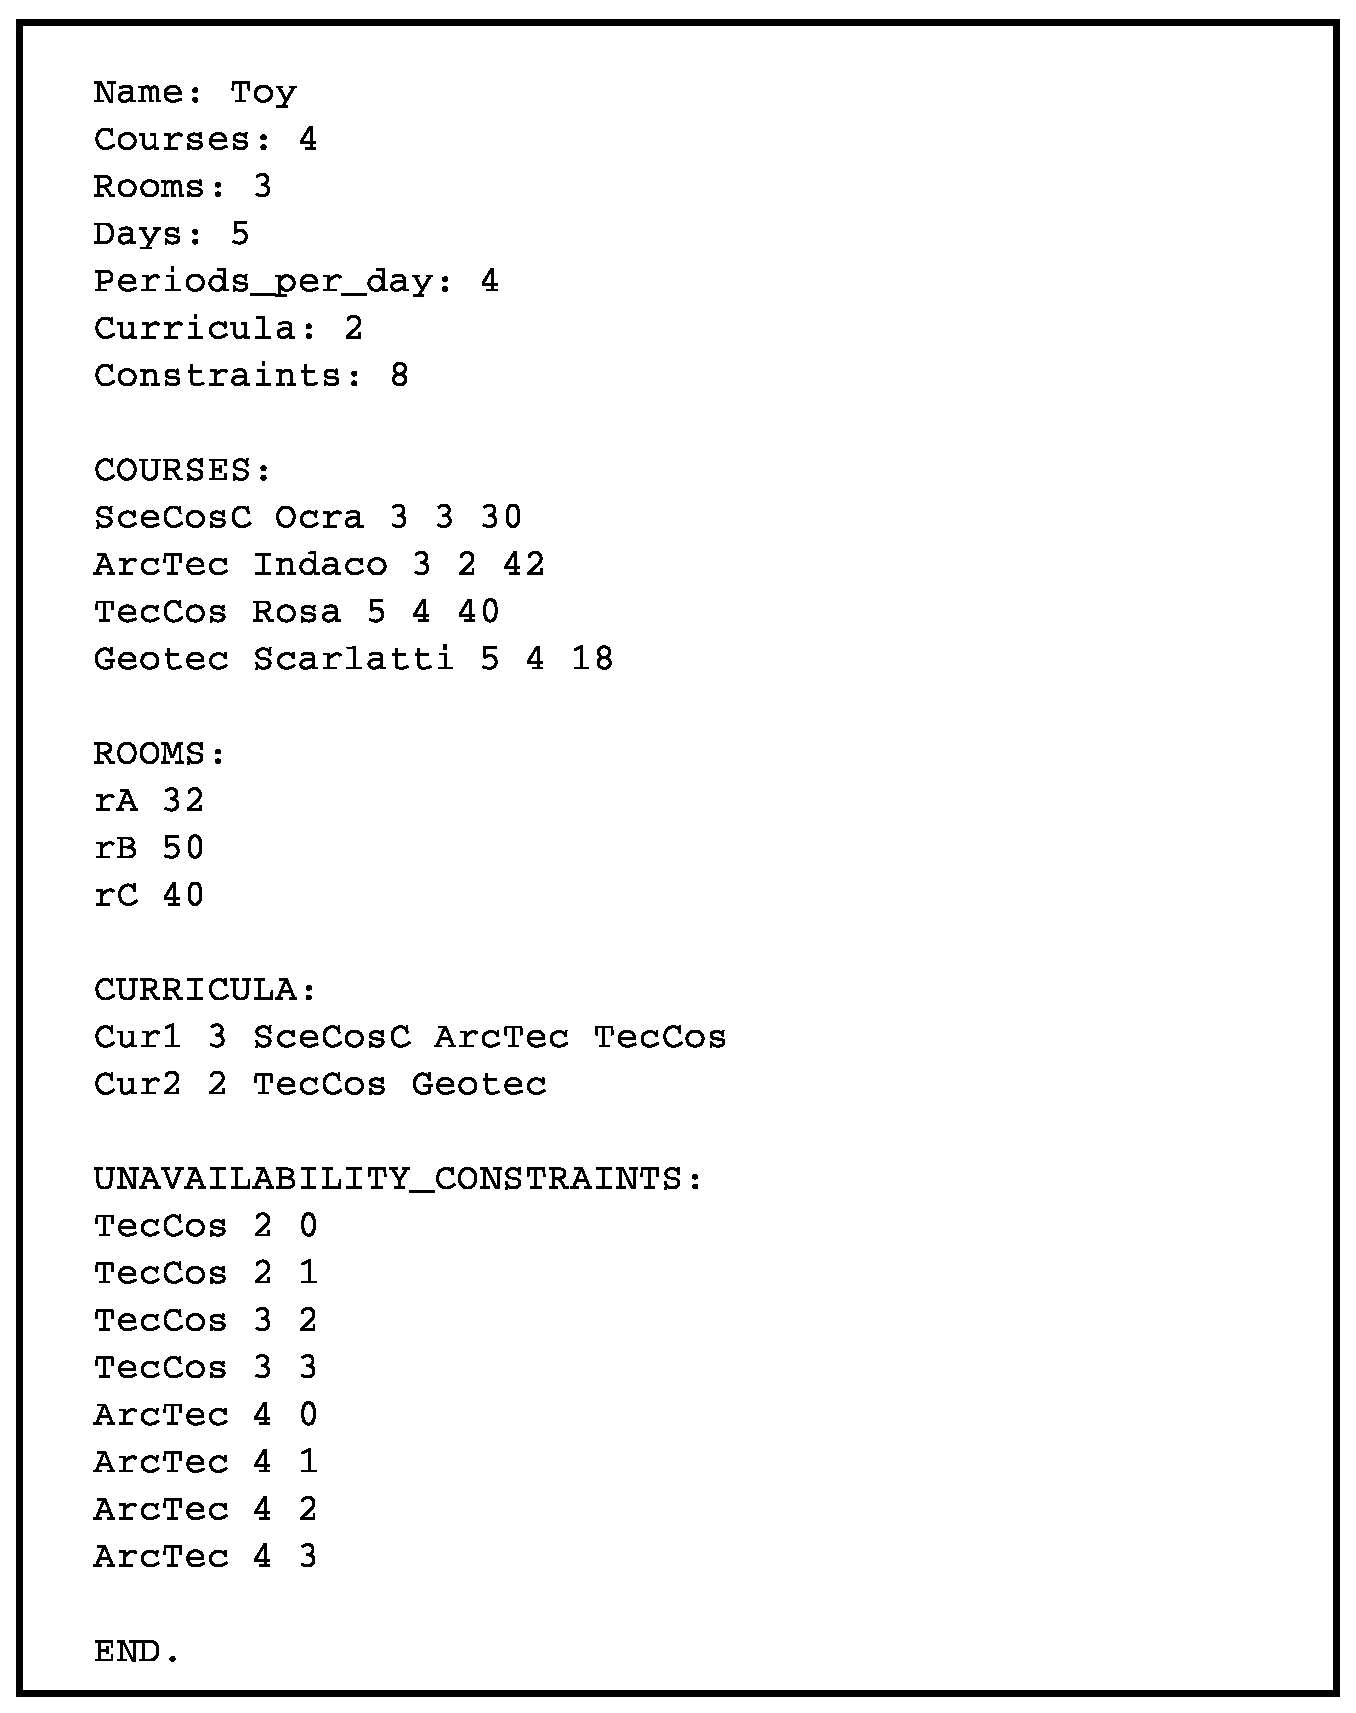
\includegraphics[width=12cm]{./InstanciaToy.eps}
 \caption{Arquivo com dados da instância {\it Toy} no formato do ITC-2007}
   \label{fig:instancia-toy}
\end{center}
\end{figure}

%\begin{boxed}
%\begin{verbatim}
%Name: Toy
%Courses: 4
%Rooms: 3
%Days: 5
%Periods_per_day: 4
%Curricula: 2
%Constraints: 8
%
%COURSES:
%SceCosC Ocra 3 3 30 
%ArcTec Indaco 3 2 42
%TecCos Rosa 5 4 40 
%Geotec Scarlatti 5 4 18 
%
%ROOMS:
%rA 32 
%rB 50 
%rC 40 
% 
%CURRICULA:
%Cur1 3 SceCosC ArcTec TecCos 
%Cur2 2 TecCos Geotec 
% 
%UNAVAILABILITY_CONSTRAINTS:
%TecCos 2 0 
%TecCos 2 1 
%TecCos 3 2 
%TecCos 3 3 
%ArcTec 4 0 
%ArcTec 4 1 
%ArcTec 4 2 
%ArcTec 4 3 
%
%END.
%\end{verbatim}

A figura \ref{fig:resposta-toy} mostra um exemplo de resposta. Informa a sala, o dia e período de cada aula.

\begin{figure}[!htb]
\begin{center}
  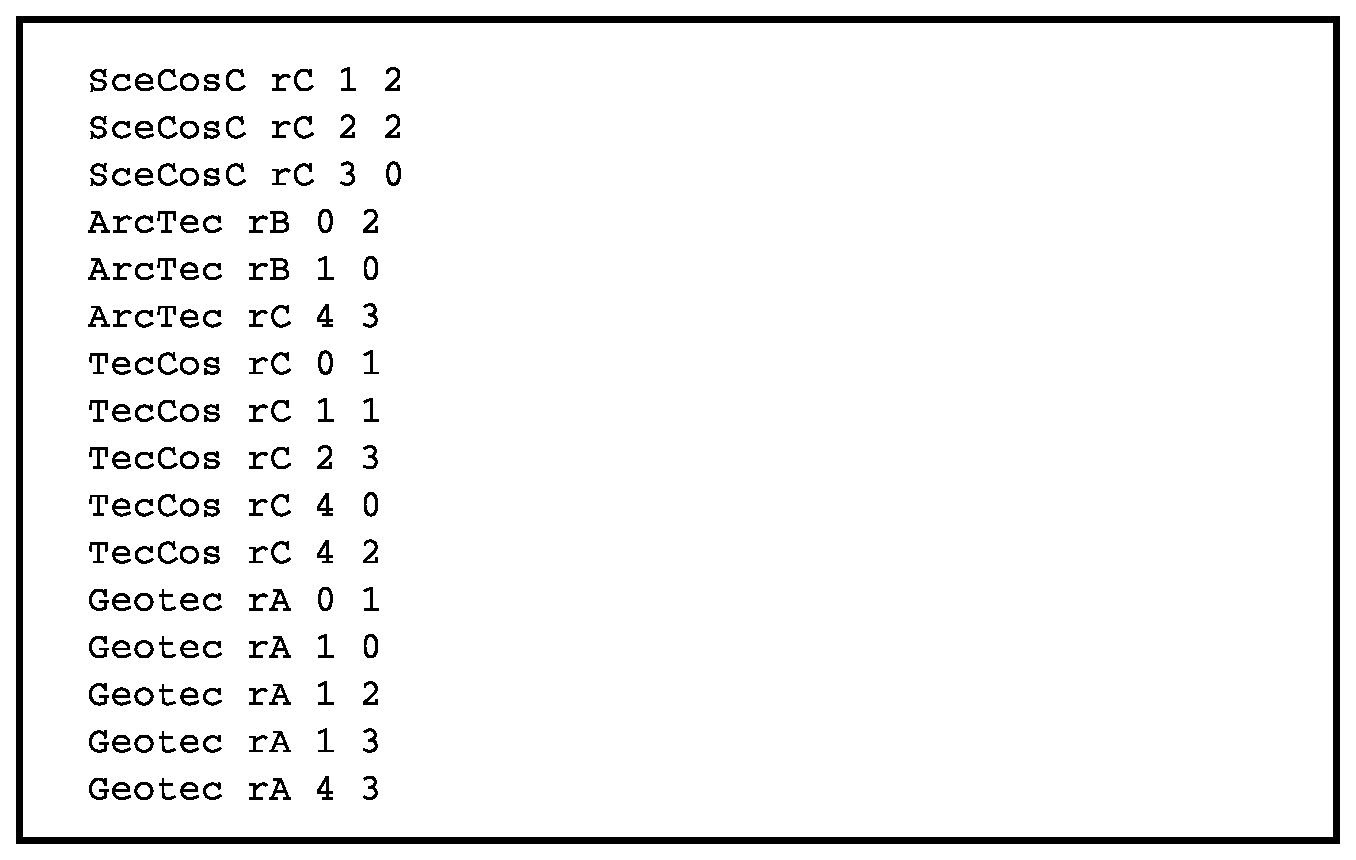
\includegraphics[width=12cm]{./RespostaToy.eps}
 \caption{Arquivo de resposta para a instância {\it Toy}}
   \label{fig:resposta-toy}
\end{center}
\end{figure}

%\begin{verbatim}
%SceCosC rC 1 2
%SceCosC rC 2 2
%SceCosC rC 3 0
%ArcTec rB 0 2
%ArcTec rB 1 0
%ArcTec rC 4 3
%TecCos rC 0 1
%TecCos rC 1 1
%TecCos rC 2 3
%TecCos rC 4 0
%TecCos rC 4 2
%Geotec rA 0 1
%Geotec rA 1 0
%Geotec rA 1 2
%Geotec rA 1 3
%Geotec rA 4 3
%\end{verbatim}

A tabela \ref{tab:solucao_toy} apresenta uma visualização desta resposta. Nesta tabela, os nomes de disciplinas  \textit{SceCosC}, \textit{ArcTec}, \textit{TecCos} e \textit{Geotec} apresentados na Figura \ref{fig:resposta-toy} são respectivamente representados por SC, AT, TC e GT.

\begin{center}
\begin{table}[!htb]
%\begin{footnotesize}
{\fontsize{9}{12} \selectfont
\begin{tabular}{|c|c|c|c|c||c|c|c|c||c|c|c|c||c|c|c|c||c|c|c|c|}\hline
 & \multicolumn{4}{|c||}{Dia 0} & \multicolumn{4}{|c||}{Dia 1}& \multicolumn{4}{|c||}{Dia 2}& \multicolumn{4}{|c||}{Dia 3}&  \multicolumn{4}{|c|}{Dia 4}\\ \hline
 & 0 & 1 & 2 & 3 & 0 & 1 & 2 & 3 & 0 & 1 & 2 & 3 & 0 & 1 & 2 & 3 & 0 & 1 & 2 & 3 \\ \hline
rA &  & GT & & & GT & & GT & GT & & &  & & & & &  &  &  &  & GT \\ \hline
rB &  &  & AT &  & AT &  &  &  &  &  &  &  &  &  &  &  &  &  &  &  \\ \hline
rC &  & TC &  &  &  & TC & SC &  &  &  & SC & TC & SC &  &  &  & TC &  & TC & AT \\ \hline
\end{tabular}
}
%\end{footnotesize}
\caption{Tabela-horário para a instância \textit{Toy}}
\label{tab:solucao_toy}
\end{table}
\end{center}

A solução ilustrada na tabela \ref{tab:solucao_toy} é inviável pois restrições fortes são violadas:

\begin{itemize}
\item RFt2 no dia 0, período 1: GT e TC estão em conflito por pertencerem ao mesmo currículo \textit{Cur2}.
\item RFt4 no dia 4, período 3: AT é indisponível neste horário.
\end{itemize}

Para corrigir estas inviabilidades podemos efetuar duas modificações na tabela. TC alocada no dia 0 é movida do período 1 para o período 0, enquanto a aula de AT alocada no dia 4 é movida para o dia 2 e período 1. O resultado destas modificações pode ser visto na tabela \ref{tab:solucao_toy_viavel}:

\begin{center}
\begin{table}[!htb]
%\begin{footnotesize}
{\fontsize{9}{12} \selectfont
\begin{tabular}{|c|c|c|c|c||c|c|c|c||c|c|c|c||c|c|c|c||c|c|c|c|}\hline
 & \multicolumn{4}{|c||}{Dia 0} & \multicolumn{4}{|c||}{Dia 1}& \multicolumn{4}{|c||}{Dia 2}& \multicolumn{4}{|c||}{Dia 3}&  \multicolumn{4}{|c|}{Dia 4}\\ \hline
 & 0 & 1 & 2 & 3 & 0 & 1 & 2 & 3 & 0 & 1 & 2 & 3 & 0 & 1 & 2 & 3 & 0 & 1 & 2 & 3 \\ \hline
rA &  & GT & & & GT & & GT & GT & & &  & & & & &  &  &  &  & GT \\ \hline
rB &  &  & AT &  & AT &  &  &  &  &  &  &  &  &  &  &  &  &  &  &  \\ \hline
rC & TC & &  &  &  & TC & SC &  &  & AT & SC & TC & SC &  &  &  & TC &  & TC &  \\ \hline
\end{tabular}
}
%\end{footnotesize}
\caption{Tabela-horário para a instância \textit{Toy} sem inviabilidades}
\label{tab:solucao_toy_viavel}
\end{table}
\end{center}

A solução ilustrada na tabela \ref{tab:solucao_toy_viavel} é viável, mas apresenta violações das seguintes restrições fracas:

\begin{itemize}
\item RFc1 para a disciplina GT: ela é lecionada em 3 dias, mas o mínimo requerido é 4.
\item RFc2: SC no dia 3 e TC no dia 4 estão isoladas, pois não possuem aulas do mesmo currículo nos períodos adjacentes. 
\item RFc3 no dia 4, período 3: a disciplina AT possui 42 alunos mas a capacidade de \textit{rC} é apenas 40.
\item RFc4 para a disciplina AT: está sendo lecionada em duas salas diferentes: \textit{rB} e \textit{rC}.
\end{itemize}

Aparentemente a tabela \ref{tab:solucao_toy_viavel} possui somente as violações citadas acima. Mas um detalhe importante é que a contagem de aulas isoladas é feita separadamente por currículo. Observando o dia 0, temos uma aula TC no período 0, uma aula GT no período 1 e uma aula AT no período 2. Quem cursa o currículo \textit{Cur2} assiste a aula TC no período 0 e a aula GT no período 1, portanto, duas aulas adjacentes. Mas quem cursa o currículo \textit{Cur1} não assiste a disciplina GT, logo, alunos deste currículo terão aula no período 0, horário vago no período 1 e depois outra aula no período 2. Portanto, são duas aulas isoladas.

Com esta observação pode se concluir que a tabela \ref{tab:solucao_toy_viavel} possui sete aulas isoladas. Totalizando todas as penalizações e lembrando que os pesos das restrições RFc1, RFc2, RFc3 e RFc4 são respectivamente 5, 2, 1 e 1, a função objetivo da solução é contabilizada pela equação \ref{calc_fo}:

\begin{equation}\label{calc_fo}
\begin{split}
f(S) &= 5\times|RFc1|_v + 2\times|RFc2|_v + |RFc3|_v + |RFc4|_v \\
f(S) &= 5 \times (4-3) + 2 \times 7 + (42-40) + (2-1) \\
f(S) &= 5 \times 1 + 2 \times 7 + 2 + 1 \\
f(S) &= 5 + 14 + 2 + 1 \\
f(S) &= 22 \\
\end{split}
\end{equation}

\chapter{Algoritmo GRASP para o problema de tabela-horário de universidades\label{cap:grasp}}

Neste capítulo será apresentado a estrutura geral da meta-heurística GRASP para problemas de otimização combinatória, além da hibridização do algoritmo com \textit{Path-Relinking}. Em seguida será descrito como ele foi aplicado no problema que está sendo abordado.

\section{Algoritmo GRASP\label{sec:estrutura_grasp}}

Um problema de otimização combinatória pode ser definido por um conjunto finito $E = \{1,...,n\}$, um conjunto de soluções viáveis $F \subseteq 2^E$ e uma função objetivo $f : 2^E \rightarrow \mathbb{R}$, todos definidos para cada problema específico. Considerando a versão de minimização, o objetivo consiste em encontrar uma solução ótima $S^* \in F$ tal que $f(S^*) \leq f(S), \forall S \in F$ \cite{Glover89}.

As meta-heurísticas são algoritmos de caráter geral que orientam uma maneira de explorar o conjunto de soluções para encontrar a solução ótima. A solução ótima não é garantida mas, em geral, as meta-heurísticas alcançam boas soluções viáveis.

A meta-heurística GRASP (\textit{Greedy Randomized Adaptive Search Procedures} - Procedimentos de busca aleatória, adaptativa e gulosa) foi introduzida por \cite{FeoRes89} para tratar o problema de cobertura de conjuntos. Desde sua proposta inicial, o GRASP já foi aplicado com sucesso em vários problemas de otimização como conjunto independente máximo \cite{FeoResSmi94}, problema quadrático de alocação \cite{LiParRes94}, satisfabilidade \cite{ResFeo96a}, planarização de grafos \cite{ResRib95}, roteamento de circuitos virtuais \cite{ResRib03a}, entre outros.

%\subsection{Estrutura básica}

O algoritmo GRASP é um procedimento com iterações independentes, onde cada iteração constrói uma solução inicial e aplica busca local para melhorá-la. A resposta final é a melhor obtida dentre as iterações. O algoritmo \ref{algoGrasp} apresenta o pseudo-código genérico do GRASP. Ao final da fase de construção inicial, pode ocorrer de a solução obtida ser inviável. Por isso um passo intermediário é previsto para reparar a solução, tornando-a viável.

\begin{algorithm}[H]
\label{algoGrasp}
\SetAlgoLined
\SetKwFunction{GeraSolucaoInicial}{GeraSolucaoInicial}
\SetKwFunction{BuscaLocal}{BuscaLocal}
\SetKwFunction{ReparaSolucao}{ReparaSolucao}
%\SetKwFunction{AtualizaPool}{AtualizaPool}
\Entrada{MaxIter}
\Saida{Solução $S^{*}$}

$f^{*} \leftarrow \infty $ \;
\Para{$i\leftarrow 1$ \Ate $MaxIter$}{
	$S \leftarrow GeraSolucaoInicial() $ \;
	\Se{$ S $ é inviável }{
		$ReparaSolucao(S) $\;
	}
	$S \leftarrow BuscaLocal(S) $ \;
	\Se{$ f(S) < f^{*} $}{
		$S^{*} \leftarrow S $ \;
		$f^{*} \leftarrow f(S) $ \;
	}
}
\caption{Estrutura básica do algoritmo GRASP}
\end{algorithm}

O método de construção da solução inicial do GRASP é guloso, aleatório e visa produzir um conjunto diversificado de soluções iniciais de boa qualidade para a busca local. Algoritmos totalmente aleatórios conseguem essa diversificação, mas as soluções em geral são ruins. Por outro lado, algoritmos gulosos tendem a gerar soluções de melhor qualidade, mas eles não conseguem produzir soluções diferentes já que a construção é sempre feita por escolhas gulosas.

O algoritmo \ref{solInicialGrasp} ilustra o procedimento de construção de uma solução genérica. Ele recebe como parâmetro um conjunto de elementos que irão compor a solução. Iterativamente um novo elemento candidato é escolhido para ser incorporado à solução. Essa escolha é gulosa aleatória. Primeiramente todos os candidatos são avaliados por uma função $g(c)$ para medir o custo de adicionar o candidato $c$ à solução parcial $S$. Com base no menor e maior custo são escolhidos os candidatos mais bem avaliados para compor a lista restrita de candidatos - LRC. Um dos candidatos é escolhido aleatoriamente desta lista. Ao ser acrescentado à solução o elemento é retirado do conjunto de candidatos. O procedimento termina quando todos os elementos foram incorporados à solução e não há mais candidatos.

O parâmetro $\alpha\, (0 \leq \alpha \leq 1)$ regula se o algoritmo será mais guloso ou mais aleatório. Quando $\alpha$ é mais próximo de zero somente os elementos com baixo custo irão entrar na LRC. Este comportamento produz soluções de boa qualidade porém pouco diversificadas. Com $\alpha$ mais próximo de um, elementos com custo mais alto poderão também entrar na LRC. Isto introduz mais aleatoriedade à solução mas, em compensação, se perde em qualidade. O ideal é encontrar um valor intermediário que permita diversificação sem prejudicar muito a qualidade de solução que será passada para a fase seguinte de busca local.

\begin{algorithm}[H]
\label{solInicialGrasp}
\SetAlgoLined
\SetKwFunction{GeraSolucaoInicial}{GeraSolucaoInicial}
\SetKwFunction{BuscaLocal}{BuscaLocal}
\SetKwFunction{PathRelinking}{PathRelinking}
\SetKwFunction{AtualizaPool}{AtualizaPool}
\Entrada{E = \{conjunto discreto finito\}}
\Saida{Solução S}

$S \leftarrow \emptyset $ \;
$C \leftarrow E $ \;
\Enqto{$|C| > 0$}{
	Para todo $c \in C$ computar o valor da função gulosa $g(c) $ \;
	$c^{min} \leftarrow min\{g(c) : c \in C\}$\;
	$c^{max} \leftarrow max\{g(c) : c \in C\}$\;
	$LRC \leftarrow \{ c \in C : g(c) \leq c^{min} + \alpha(c^{max} - c^{min}) \} $ \;
	Escolha aleatoriamente $c' \in LRC $ \;
	$S \leftarrow S \bigcup \{ c' \} $\;
	$C \leftarrow C - \{ c' \}$ \;
}
\caption{Algoritmo guloso aletório para construção da solução inicial do GRASP}
\end{algorithm}

Para encontrar boas soluções, uma meta-heurística precisa ter duas características importantes: diversificação e intensificação. A primeira refere-se à capacidade de explorar bem o espaço de soluções e não ficar preso a mínimos locais (ou máximos locais em problemas de maximização). A intensificação é necessária para explorar bem uma região de mínimo local, dado que o mínimo global necessariamente também é um mínimo local.

No GRASP a diversificação é feita pela independência das iterações e pela aleatoriedade introduzida na solução inicial, enquanto a intensificação é feita pela busca local. Nesta fase a solução inicial é melhorada explorando sua vizinhança na busca de soluções melhores.

O GRASP não especifica qual a estratégia de busca local deve ser utilizada. No trabalho de \cite{FeoResSmi94} a busca local implementada é conhecida como \textit{Hill Climbing}. É uma estratégia simples em que se explora a vizinhança enquanto são encontradas soluções melhores. Em \cite{Souza:2004:GSA} por exemplo, os autores utilizaram a Busca Tabu para compor a fase de melhoramento da solução inicial.

\section{GRASP + \textit{Path-Relinking}}

A heurística \textit{Path-Relinking} (PR) (religamento de caminhos) foi originalmente proposta por \cite{Glover96tabusearch} como uma estratégia de intensificação na Busca Tabu. A primeira proposta de uso do \textit{Path-Relinking} no GRASP foi feita por \cite{Laguna99graspand}. Essa hibridização tenta resolver uma deficiência do GRASP que é ausência de memorização entre as iterações.

A idéia básica do \textit{Path-Relinking} é traçar um caminho ligando duas soluções que são chamadas de inicial e alvo. Para gerar este caminho, sucessivamente são inseridos atributos da solução alvo na solução inicial para que ela fique a cada iteração mais parecida com a solução alvo. A cada atributo inserido uma solução diferente é obtida. A melhor solução obtida no caminho é a resposta do algoritmo. Desta forma, o religamento de caminhos pode ser visto como uma estratégia que procura incorporar atributos de soluções de alta qualidade.

De forma genérica, o caminho percorrido pelo \textit{Path-Relinking} é ilustrado na figura \ref{fig:path-relinking-generico}. A partir de uma solução inicial um caminho é percorrido até a solução alvo, gerando novas soluções intermediárias que podem ser melhores que a inicial e a alvo. Em cada iteração, verifica-se quais atributos estão diferentes na solução inicial e alvo. No exemplo da figura \ref{fig:path-relinking-generico} são quatro diferenças, por isso quatro soluções podem ser geradas a partir da solução inicial. Opta-se por uma delas e continua a busca a partir da escolhida até se chegar na solução alvo. A quantidade de iterações necessárias para realizar o percurso é no máximo a quantidade de diferenças entre as duas soluções.

\begin{figure}[!htb]
\begin{center}
  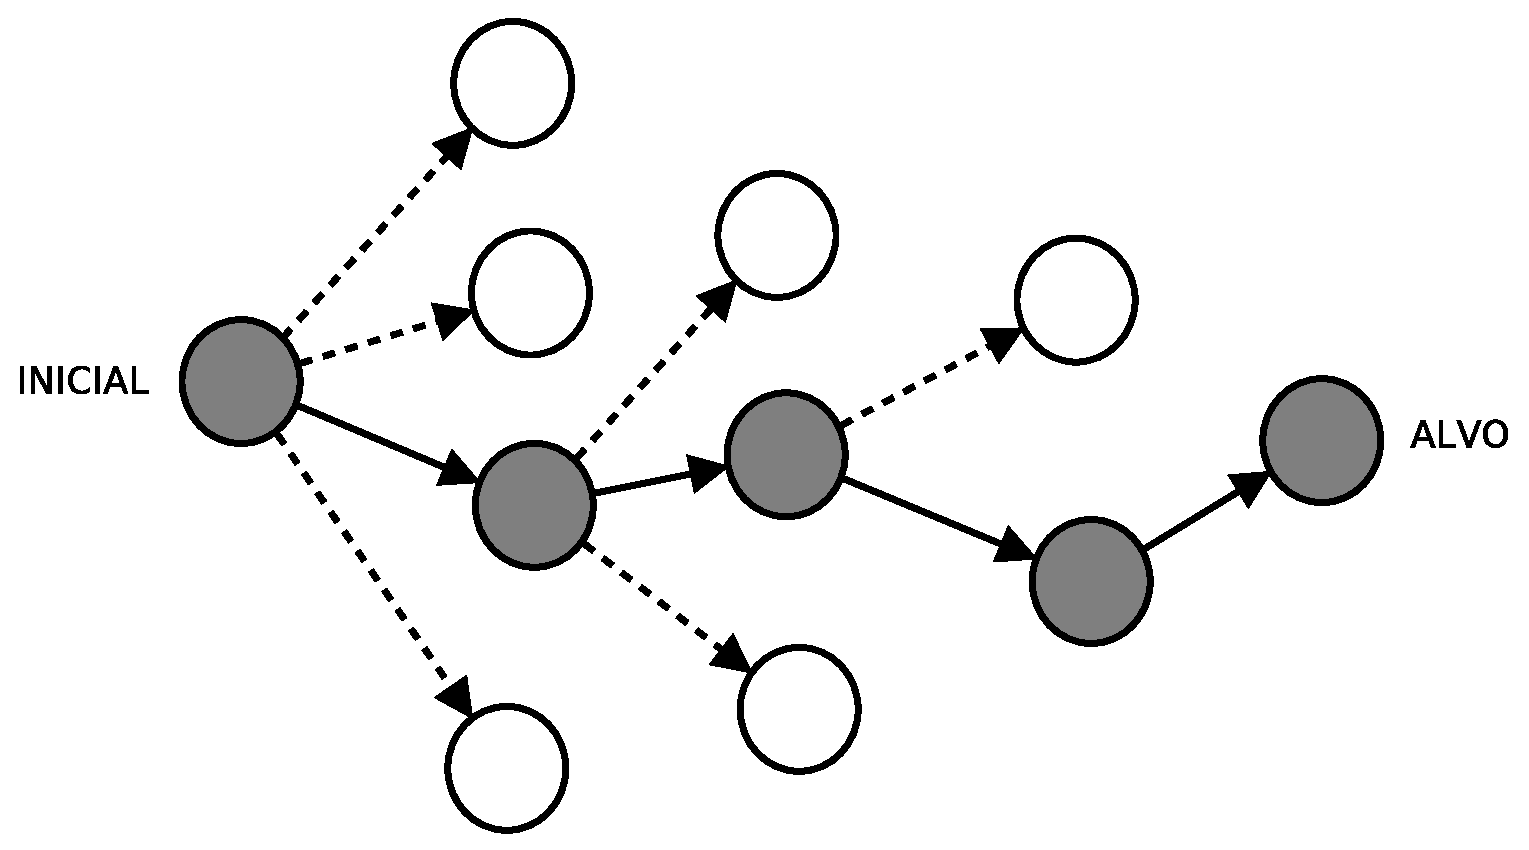
\includegraphics[width=12cm]{./PRgenerico.eps}
 \caption{Explorando soluções com \textit{Path-Relinking}}
   \label{fig:path-relinking-generico}
\end{center}
\end{figure}

A figura \ref{fig:path-relinking} ilustra o \textit{Path-Relinking} para o caso específico de tabela-horário. Nas tabelas fictícias da figura \ref{fig:path-relinking} estão alocadas 7 aulas. Comparando as tabelas inicial e alvo percebe-se que 4 aulas estão na mesma posição e 3 em posições diferentes, destacadas com um círculo. No caminho percorrido, a cada nova tabela uma posição é corrigida. Todas as tabelas intermediárias são avaliadas pois podem ter melhor função objetivo.

O caminho escolhido não é único. No exemplo da figura \ref{fig:path-relinking}, dentre as três aulas que estão em posições divergentes da solução alvo, optou-se por corrigir primeiro a aula da disciplina \texttt{AT}. Mas também poderia ter começado por outra aula. Em geral, é mais comum escolher o passo que irá produzir a melhor tabela-horário (estratégia gulosa), mas pode ser introduzida aleatoriedade nesta escolha, assim como é feito na construção da solução inicial.

\begin{figure}[!htb]
\begin{center}
  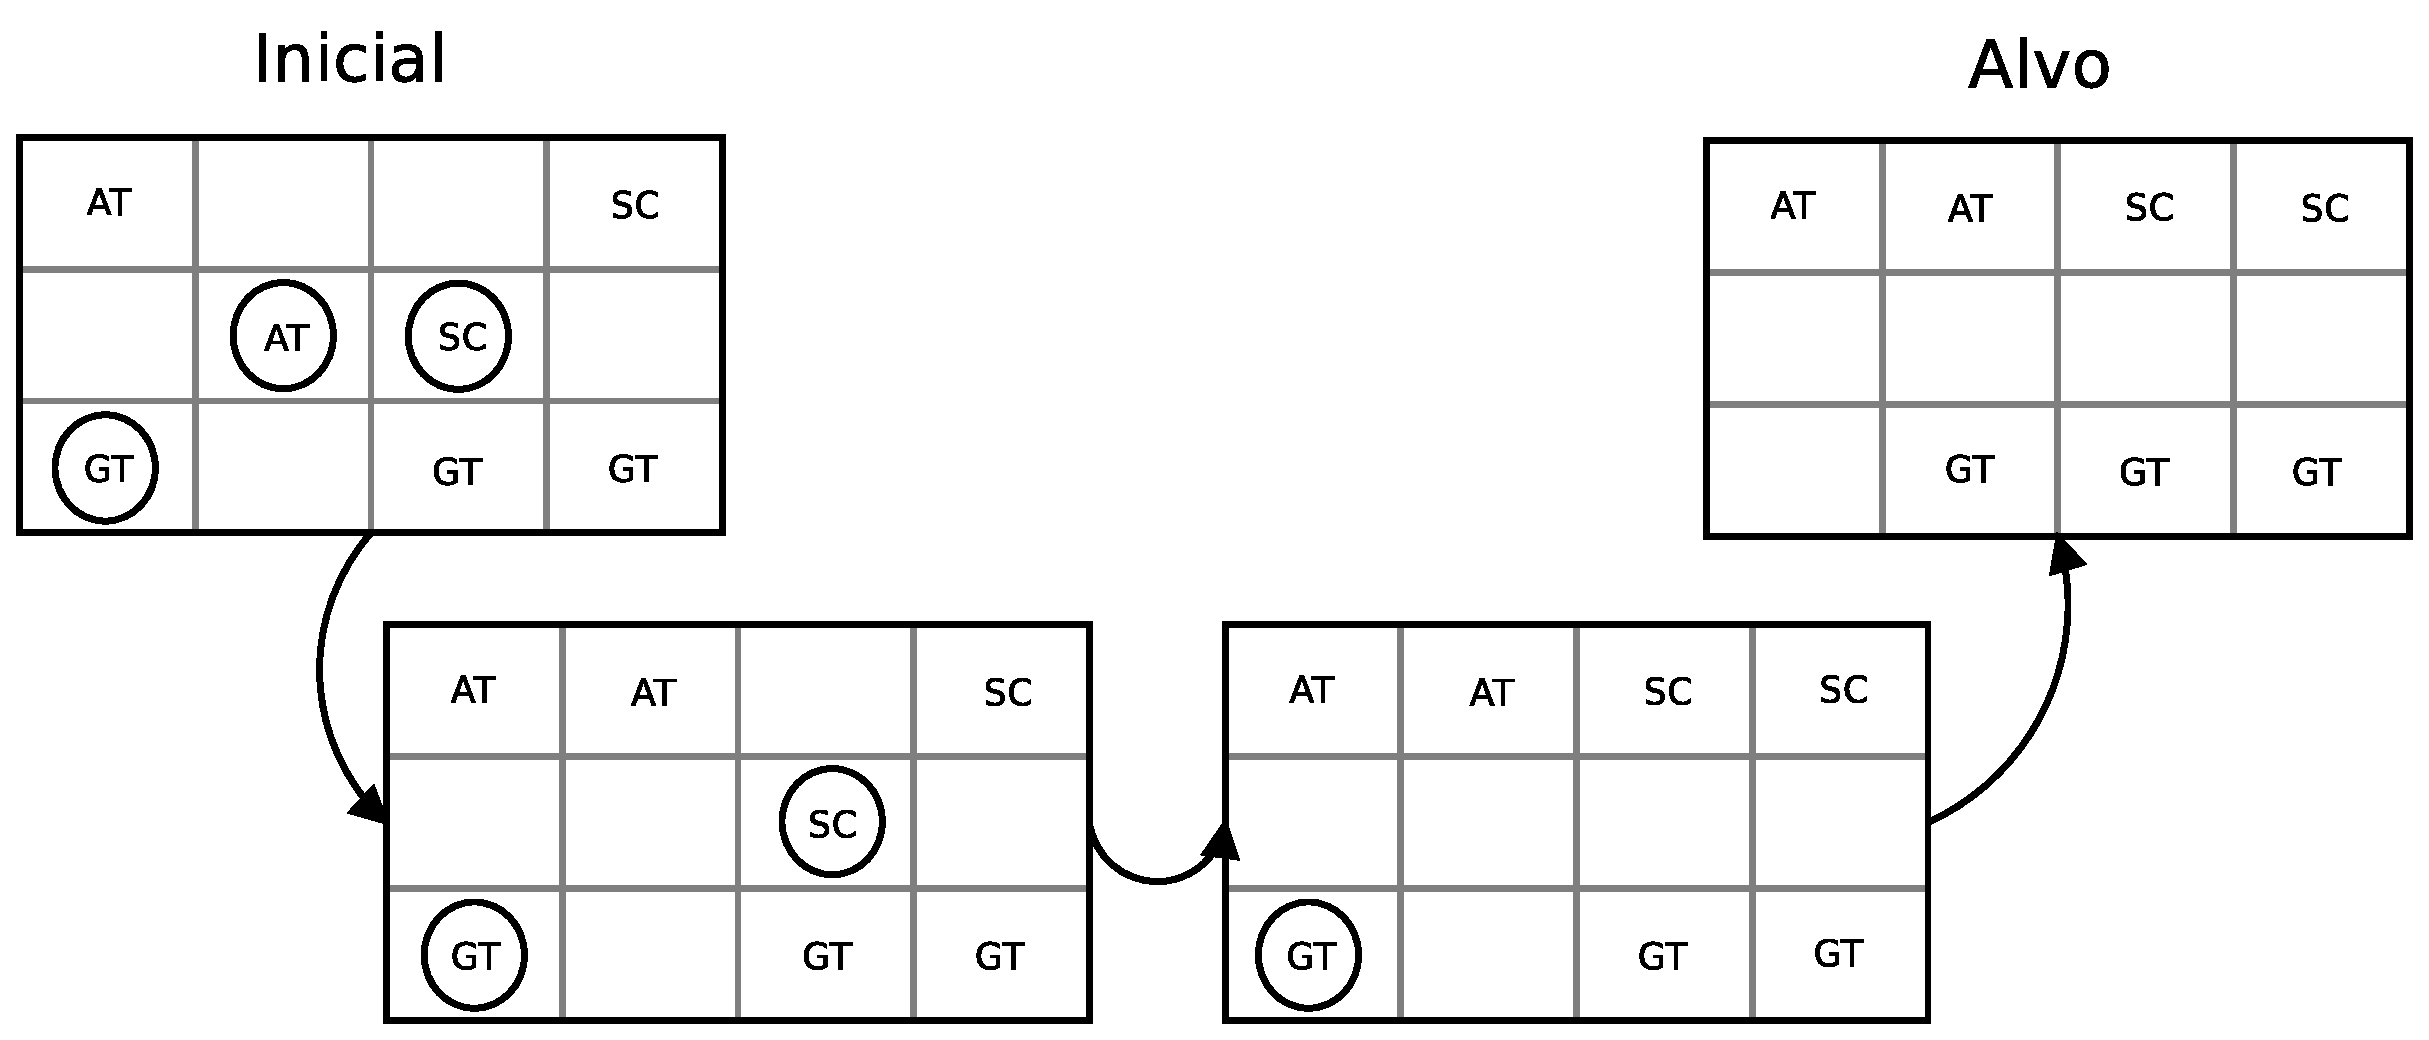
\includegraphics[width=14cm]{./PR.eps}
 \caption{Trajetória do {\it Path-relinking} ligando duas tabelas}
   \label{fig:path-relinking}
\end{center}
\end{figure}

A quantidade de iterações necessárias para percorrer o caminho é no máximo a quantidade de diferenças entre as soluções inicial e alvo. Isso acontece porque cada iteração corrige uma diferença sem acrescentar outra, dado que o procedimento não altera as aulas que já estão em suas posições corretas na tabela-horário.

O pseudo-código do algoritmo \ref{path-relinking} ilustra o PR aplicado ao par de soluções $x_i$ (inicial) e $x_a$ (alvo). Nas linhas 1 e 2 são inicializadas as variáveis que guardam o melhor valor de função objetivo encontrado e a solução que produziu este valor. Na linha 4 o procedimento computa a diferença simétrica $\Delta(x_i,x_a)$ entre as duas soluções, isto é, o conjunto mínimo de movimentos necessários para alcançar $x_a$ a partir de $x_i$. Um caminho de soluções é gerado ligando $x_i$ e $x_a$. A melhor solução $x^*$ no caminho é a resposta do algoritmo. Em cada iteração, o procedimento examina todos os movimentos $m \in \Delta(x, x_a)$ a partir da solução corrente $x$ e seleciona aquele que resulta no custo de solução menor, isto é, aquele que minimiza $f(x \oplus m)$, onde $x \oplus m$ é a solução resultante da aplicação do movimento $m$ à solução $x$ (linhas 5 a 13). O melhor movimento $m^*$ produz a solução $x \oplus m^*$. O conjunto de movimentos possíveis é atualizado na linha 7. Se for o caso, a melhor solução $x^*$ é atualizada nas linhas 9 a 11. O procedimento termina quando $x_a$ é alcançada, ou seja, $\Delta(x, x_a) = \emptyset$.

\begin{algorithm}[H]
\label{path-relinking}
\SetAlgoLined
\SetKwFunction{GeraSolucaoInicial}{GeraSolucaoInicial}
\SetKwFunction{BuscaLocal}{BuscaLocal}
\SetKwFunction{PathRelinking}{PathRelinking}
\SetKwFunction{AtualizaPool}{AtualizaPool}
\Entrada{Solução inicial $x_i$, solução alvo $x_a$}
\Saida{Melhor solução $x^{*}$ no caminho de $x_i$ para $x_a$}

$f^{*} \leftarrow min \{ f(x_i), f(x_a) \} $ \;
$x^{*} \leftarrow argmin \{ f(x_i), f(x_a) \} $ \;
$x \leftarrow x_i $ \;
Compute as diferenças simétricas $\Delta(x,x_a) $ \;
\Enqto{$\Delta(x,x_a) \neq \emptyset $}{
	$m^* \leftarrow argmin  \{ f(x \oplus m) : m \in \Delta(x,x_a) \}$ \;
	$ \Delta(x \oplus m^*,x_a) \leftarrow \Delta(x,x_a) - \{ m^* \}$ \;
	$ x \leftarrow x \oplus m^* $ \;
	\Se{$ f(x) < f^* $}{
		$f^* \leftarrow f(x) $ \;
		$x^* \leftarrow x $ \;
	}
}
\caption{Algoritmo \textit{Path-Relinking}}
\end{algorithm}

O PR pode ser visto com uma estratégia de busca local mais restrita, onde os movimentos aplicados são mais específicos.

De acordo com \cite{Resende05graspwith}, \textit{Path-Relinking} é uma estratégia adicionada ao algoritmo básico do GRASP, proporcionando melhoras tanto no tempo computacional quanto na qualidade de solução. Para aplicar o PR é necessário que o GRASP mantenha um conjunto de soluções elites com as melhores soluções encontradas durante a execução do algoritmo. \cite{Resende05graspwith} também descrevem duas formas de inserir o PR no GRASP:

\begin{itemize}

\item PR é aplicado entre todos os pares de soluções elite. Pode ser feito periodicamente durante as iterações do GRASP ou no final da execução como uma pós-otimização.

\item PR é aplicado como estratégia de intensificação em cada mínimo local obtido pela busca local.

\end{itemize}

O algoritmo \ref{algoGraspComPathRelinking} ilustra as duas estratégias embutidas na versão básica do GRASP. O \textit{Path-Relinking} é aplicado entre duas soluções $x$ e $y$: $x$ é um ótimo local obtido na busca local e $y$ é uma solução escolhida aleatoriamente do conjunto de soluções elite, denominado Elite. Esse procedimento é aplicado somente a partir da segunda iteração pois na primeira o conjunto Elite está vazio. O número de elementos desse conjunto é limitado por $MaxElite$, parâmetro do algoritmo.

Ao final de cada iteração o conjunto Elite é atualizado. Todo ótimo local obtido é candidato a entrar no conjunto. Se ele já tem $MaxElite$ soluções, o candidato só irá entrar se for diferente das soluções presentes e melhor que ao menos uma delas. O controle de entrada e saída de soluções no conjunto Elite é feito pelo procedimento $AtualizaElite$.

Ao final das iterações ocorre a pós-otimização, em que se aplica \textit{Path-Relinking} entre as soluções do conjunto Elite, duas as duas. A melhor solução obtida é a resposta do algoritmo.

\begin{algorithm}[H]
\label{algoGraspComPathRelinking}
\SetAlgoLined
\SetKwFunction{GeraSolucaoInicial}{GeraSolucaoInicial}
\SetKwFunction{BuscaLocal}{BuscaLocal}
\SetKwFunction{PathRelinking}{PathRelinking}
\SetKwFunction{AtualizaPool}{AtualizaPool}
\Entrada{MaxIter, MaxElite}
\Saida{Melhor Solução $S^{*}$}

$f^{*} \leftarrow \infty $ \;
$Elite \leftarrow \emptyset $ \;
\Para{$i\leftarrow 1$ \Ate $MaxIter$}{
	$S \leftarrow GeraSolucaoInicial() $ \;
	$S \leftarrow BuscaLocal(S) $ \;
	\Se{$ i \geq 2 $}{
		Selecione aleatoriamente $S_{elite} \in Elite $ \;
		$S \leftarrow PathRelinking(S, S_{elite}) $ \;
	}
	\Se{$ f(S) < f^{*} $}{
		$S^{*} \leftarrow S $ \;
		$f^{*} \leftarrow f(S) $ \;
	}
	$AtualizaElite(S, Elite)$ \;
}
$S^* = PosOtimizacao(Elite)$ \;
\caption{GRASP com \textit{Path-Relinking} para intensificação e pós-otimização}
\end{algorithm}

\section{GRASP + PR para o ITC-2007}

Nesta seção apresentamos a implementação do algoritmo \ref{algoGraspComPathRelinking} adaptado ao problema de tabela-horário modelado pela terceira formulação do ITC-2007 apresentada na seção \ref{sec:formulacao}. A adaptação do algoritmo \ref{algoGraspComPathRelinking} ao problema foi realizada em três etapas principais: geração de solução inicial (linha 4), busca local (linha 5) e \textit{Path-Relinking} (linha 8).

\subsection{Geração de tabela-horário inicial}

O objetivo da etapa de construção inicial é produzir uma tabela-horário viável, e se possível, com poucas violações das restrições fracas. O GRASP não exige que a solução inicial seja viável, mas foi decidido implementar desta forma para que nas fases seguintes o algoritmo se concentre apenas na eliminação das violações das restrições fracas. A contagem de violações fortes e fracas requer certo esforço computacional. Garantindo que as soluções são viáveis, a etapa de busca local não necessita contar as violações fortes.

Partindo de uma tabela-horário vazia, as aulas são acrescentadas uma a uma até que todas estejam alocadas. A escolha é tanto gulosa (para produzir soluções de boa qualidade) quanto aleatória (para produzir soluções diversificadas).

Com intuito de obter uma solução viável, é adotada uma estratégia de alocar as aulas mais conflitantes primeiro. Poucos horários são viáveis para as disciplinas mais conflitantes, portanto, é melhor alocá-las quando a tabela está mais vazia. Para medir se uma aula é mais conflitante que outra são contados quantos horários disponíveis são adequados para alocar a aula da disciplina. Esta contagem envolve:

\begin{itemize}

\item contar a quantidade de horários disponíveis (desocupados)
\item retirar os horários em o que o professor da disciplina já leciona alguma aula;
\item retirar os horários em que estão alocadas disciplinas do mesmo currículo;
\item retirar os horários que são indisponíveis para a disciplina segundo a restrição de indisponibilidade.

\end{itemize}

Em cada iteração, a aula mais difícil (a que possui menos horários viáveis) é escolhida para ser alocada. Existem diferentes combinações de horários e salas para a alocação. Os custos de todas essas combinações são calculados levando-se em conta as penalizações das restrições fracas. As combinações que possuem horários inviáveis são descartadas. Com base no menor e maior custo de adição de um elemento à solução ($c^{min}$ e $c^{max}$) é construída a lista restrita de candidatos (LRC). Pertencem à LRC as aulas cujos custos estejam no intervalo \begin{math} [c^{min}, c^{min}+\alpha(c^{max} - c^{min})]\end{math}. Uma aula é escolhida aleatoriamente da LRC e acrescentada à solução.

É possível que em alguns casos, ao escolher uma aula para alocar, não haja um horário que mantenha a viabilidade da solução. Para contornar esta situação foi implementado um procedimento denominado explosão. É uma estratégia que retira da tabela uma aula alocada anteriormente para abrir espaço para a aula que não está sendo possível alocar. A aula retirada volta para o conjunto de aulas não alocadas.

A primeira estratégia de explosão utilizada consiste em escolher o horário que possui menos disciplinas conflitantes e retirar todas elas da tabela. Essa estratégia não se mostrou muito eficaz pois favoreceu a formação de ciclagem no algoritmo, isto é, retirando uma aula e alocando outra, mas posteriormente fazendo o inverso, já que o horário escolhido era quase sempre o mesmo.

Uma estratégia mais eficaz é a escolha de um horário (dentre os viáveis) aleatoriamente, ao invés de selecionar aquele com menos aulas conflitantes. Testes mostraram que essa estratégia evita o problema de ciclagem.

O algoritmo \ref{solInicialGrasp-ITC2007} ilustra o procedimento de geração de uma tabela-horário inicial. Ele recebe como parâmetro as aulas das disciplinas a serem alocadas na tabela que inicialmente é vazia (linha 1). Para facilitar a obtenção da aula mais conflitante durante as iterações é criada uma lista de aulas não alocadas (linha 2). Esta lista é ordenada de forma decrescente pela quantidade de conflitos, portanto a aula na primeira posição da lista é a mais conflitante.

A cada passo da construção da solução inicial a aula mais conflitante que ainda não foi alocada é selecionada na linha 5. Em seguida é verificado em quais horários pode ser alocada a aula sem gerar inviabilidades (linha 6). Esses horários formam o conjunto $H$. Se não houver horário disponível ocorre a explosão (linhas 7 a 10), portanto, $H$ terá pelo menos um horário e será possível fazer a alocação. Os horários disponíveis são combinados com todas as salas e é feita uma avaliação do custo de alocação da aula na respectiva sala e horário (linha 11). Com base nos custos é construída a lista restrita de candidatos (linhas 12 a 14). A aula é então inserida na tabela numa posição escolhida aleatoriamente da LRC. A lista de aulas não alocadas é atualizada e ordenada novamente (linhas 17 e 18). Essa ordenação é necessária porque a última aula alocada poderá gerar conflitos com as aulas que ainda serão alocadas. O procedimento termina quando todas aulas estão inseridas na tabela-horário.

\begin{algorithm}[H]
\label{solInicialGrasp-ITC2007}
\SetAlgoLined
\SetKwFunction{GeraSolucaoInicial}{GeraSolucaoInicial}
\SetKwFunction{BuscaLocal}{BuscaLocal}
\SetKwFunction{PathRelinking}{PathRelinking}
\SetKwFunction{OrdenaAulasPorDificuldade}{OrdenaAulasPorDificuldade}
\Entrada{A = \{conjunto de aulas\}, S = \{conjunto de salas\}, $\alpha$}
\Saida{Tabela-horário T}

$T \leftarrow \emptyset $ \;
$ListaNaoAlocadas \leftarrow GeraListaNaoAlocadas(A) $ \;
$OrdenaAulasPorConflitos(ListaNaoAlocadas) $ \;
\Enqto{$|ListaNaoAlocadas| > 0$}{
	$ a \leftarrow ListaNaoAlocadas[0] $ \;
	$H \leftarrow \{ h \text{ tal que } h $ é viável para $ a \}$ \;
	\Se{$ H = \emptyset $}{
		ExplodeSolucao(T, a) \;
		$H \leftarrow \{ h \text{ tal que } h $ é viável para $ a \}$ \;
	}
	Para todo $ (s, h) \in S \times H, T[s, h] = \emptyset $, computar o custo de alocação $f(a,s,h) $ \;
	$c^{min} \leftarrow min\{f(a,s,h) : (s, h) \in S \times H\}$\;
	$c^{max} \leftarrow max\{f(a,s,h) : (s, h) \in S \times H\}$\;
	$LRC \leftarrow \{ (s,h) \in S \times H : f(a,s,h) \leq c^{min} + \alpha(c^{max} - c^{min}) \} $ \;
	Escolha aleatoriamente $(s',h') \in LRC $ \;
	$T[s',h'] = a $\;
	$RetiraAula(ListaNaoAlocadas, a) $ \;
	$OrdenaAulasPorConflitos(ListaNaoAlocadas) $ \;
}
\caption{Algoritmo construtivo para geração de tabela-horário inicial}
\end{algorithm}

A figura \ref{fig:solucao-inicial} ilustra uma iteração do algoritmo \ref{solInicialGrasp-ITC2007} aplicado na instância \textit{Toy}, que foi descrita na seção \ref{sec:formulacao}. A instância foi simplificada para facilitar a ilustração. São apenas três dias de aula, cada um com dois horários. As disciplinas \textit{SceCosC}, \textit{ArcTec}, \textit{TecCos} e \textit{GeoTec} possuem respectivamente 1, 1, 2 e 2 aulas semanais. Vamos supor também que as duas aulas de \textit{GeoTec} devem acontecer em dois dias diferentes.

Na ilustração da figura \ref{fig:solucao-inicial} quatro aulas já foram alocadas e a próxima é uma aula da disciplina \textit{GeoTec} (GT), pois é a primeira da lista de não-alocadas. O primeiro passo é verificar se há posições viáveis para inserir a aula. Os horários $h0$ e $h1$ são descartados pois neles há aulas conflitantes da disciplina \textit{TecCos} por serem do mesmo currículo. O horário $h3$ também é descartado pois já possui uma aula de GT. O conjunto de horários viáveis é portanto $H = \{h2, h4, h5 \}$. A aula GT pode ser alocada em qualquer um dos horários pertencentes a $H$, pois a viabilidade da tabela fica mantida, uma vez que os horários inviáveis foram descartados.

 Todas as salas que estiverem desocupadas nestes horários são avaliadas para montar a lista restrita de candidatos. Os custos de cada posição são calculados levando em consideração as penalizações das restrições fracas. Exemplificando duas opções:

\begin{itemize}

\item (rA, h2):
	\begin{itemize}
	\item Capacidade de Sala: Não há penalização, pois rA possui 32 assentos e GT 18 alunos.
	\item Estabilidade de Sala: Há penalização, pois uma aula de GT já está alocada em rC. Assim GT passaria a ter aulas em duas salas diferentes, logo, penalização de 1 unidade.
	\item Aulas Isoladas: Não há penalização, pois em $h3$ há uma aula do mesmo currículo.
	\item Dias Mínimos de Trabalho: Há penalização, pois GT teria aula em apenas um dia, enquanto o mínimo requerido são dois. Penalização de 1 unidade com peso 5.
	\item Custo Total: 6.
	\end{itemize}

\item (rC, h5):
	\begin{itemize}
	\item Capacidade de Sala: Não há penalização, pois rC possui 40 assentos e GT 18 alunos.
	\item Estabilidade de Sala: Não há penalização, pois GT continuaria usando apenas uma sala.
	\item Aulas Isoladas: Há penalização, pois não há uma aula do mesmo currículo em períodos adjacentes do mesmo dia. Penalização de 1 unidade com peso 2.
	\item Dias Mínimos de Trabalho: Não há penalização, pois GT teria aulas em dois dias diferentes.
	\item Custo Total: 2.
	\end{itemize}
\end{itemize}

Avaliando todas as combinações de sala e horários disponíveis, temos o menor custo $c^{min} = 2$ e o máximo $c^{max} = 6$. As combinações que irão para a lista restrita de candidatos são as que tem custo no intervalo \begin{math} [c^{min}; c^{min}+\alpha(c^{max} - c^{min})]\end{math}. Usando $\alpha=0.15$, teremos um intervalo \begin{math} [2;\, 2+0,15(6 - 2)]\end{math}, ou \begin{math} [2;\,2,6]\end{math}. Somente as combinações que tem custo neste intervalo são ($rC,h4$) e ($rC,h5$). Escolhendo aleatoriamente a segunda, GT será alocada na sala $rC$ e horário $h5$. Consequentemente, GT sai da lista de aulas não-alocadas restando apenas SC.

\begin{figure}[!htb]
\begin{center}
  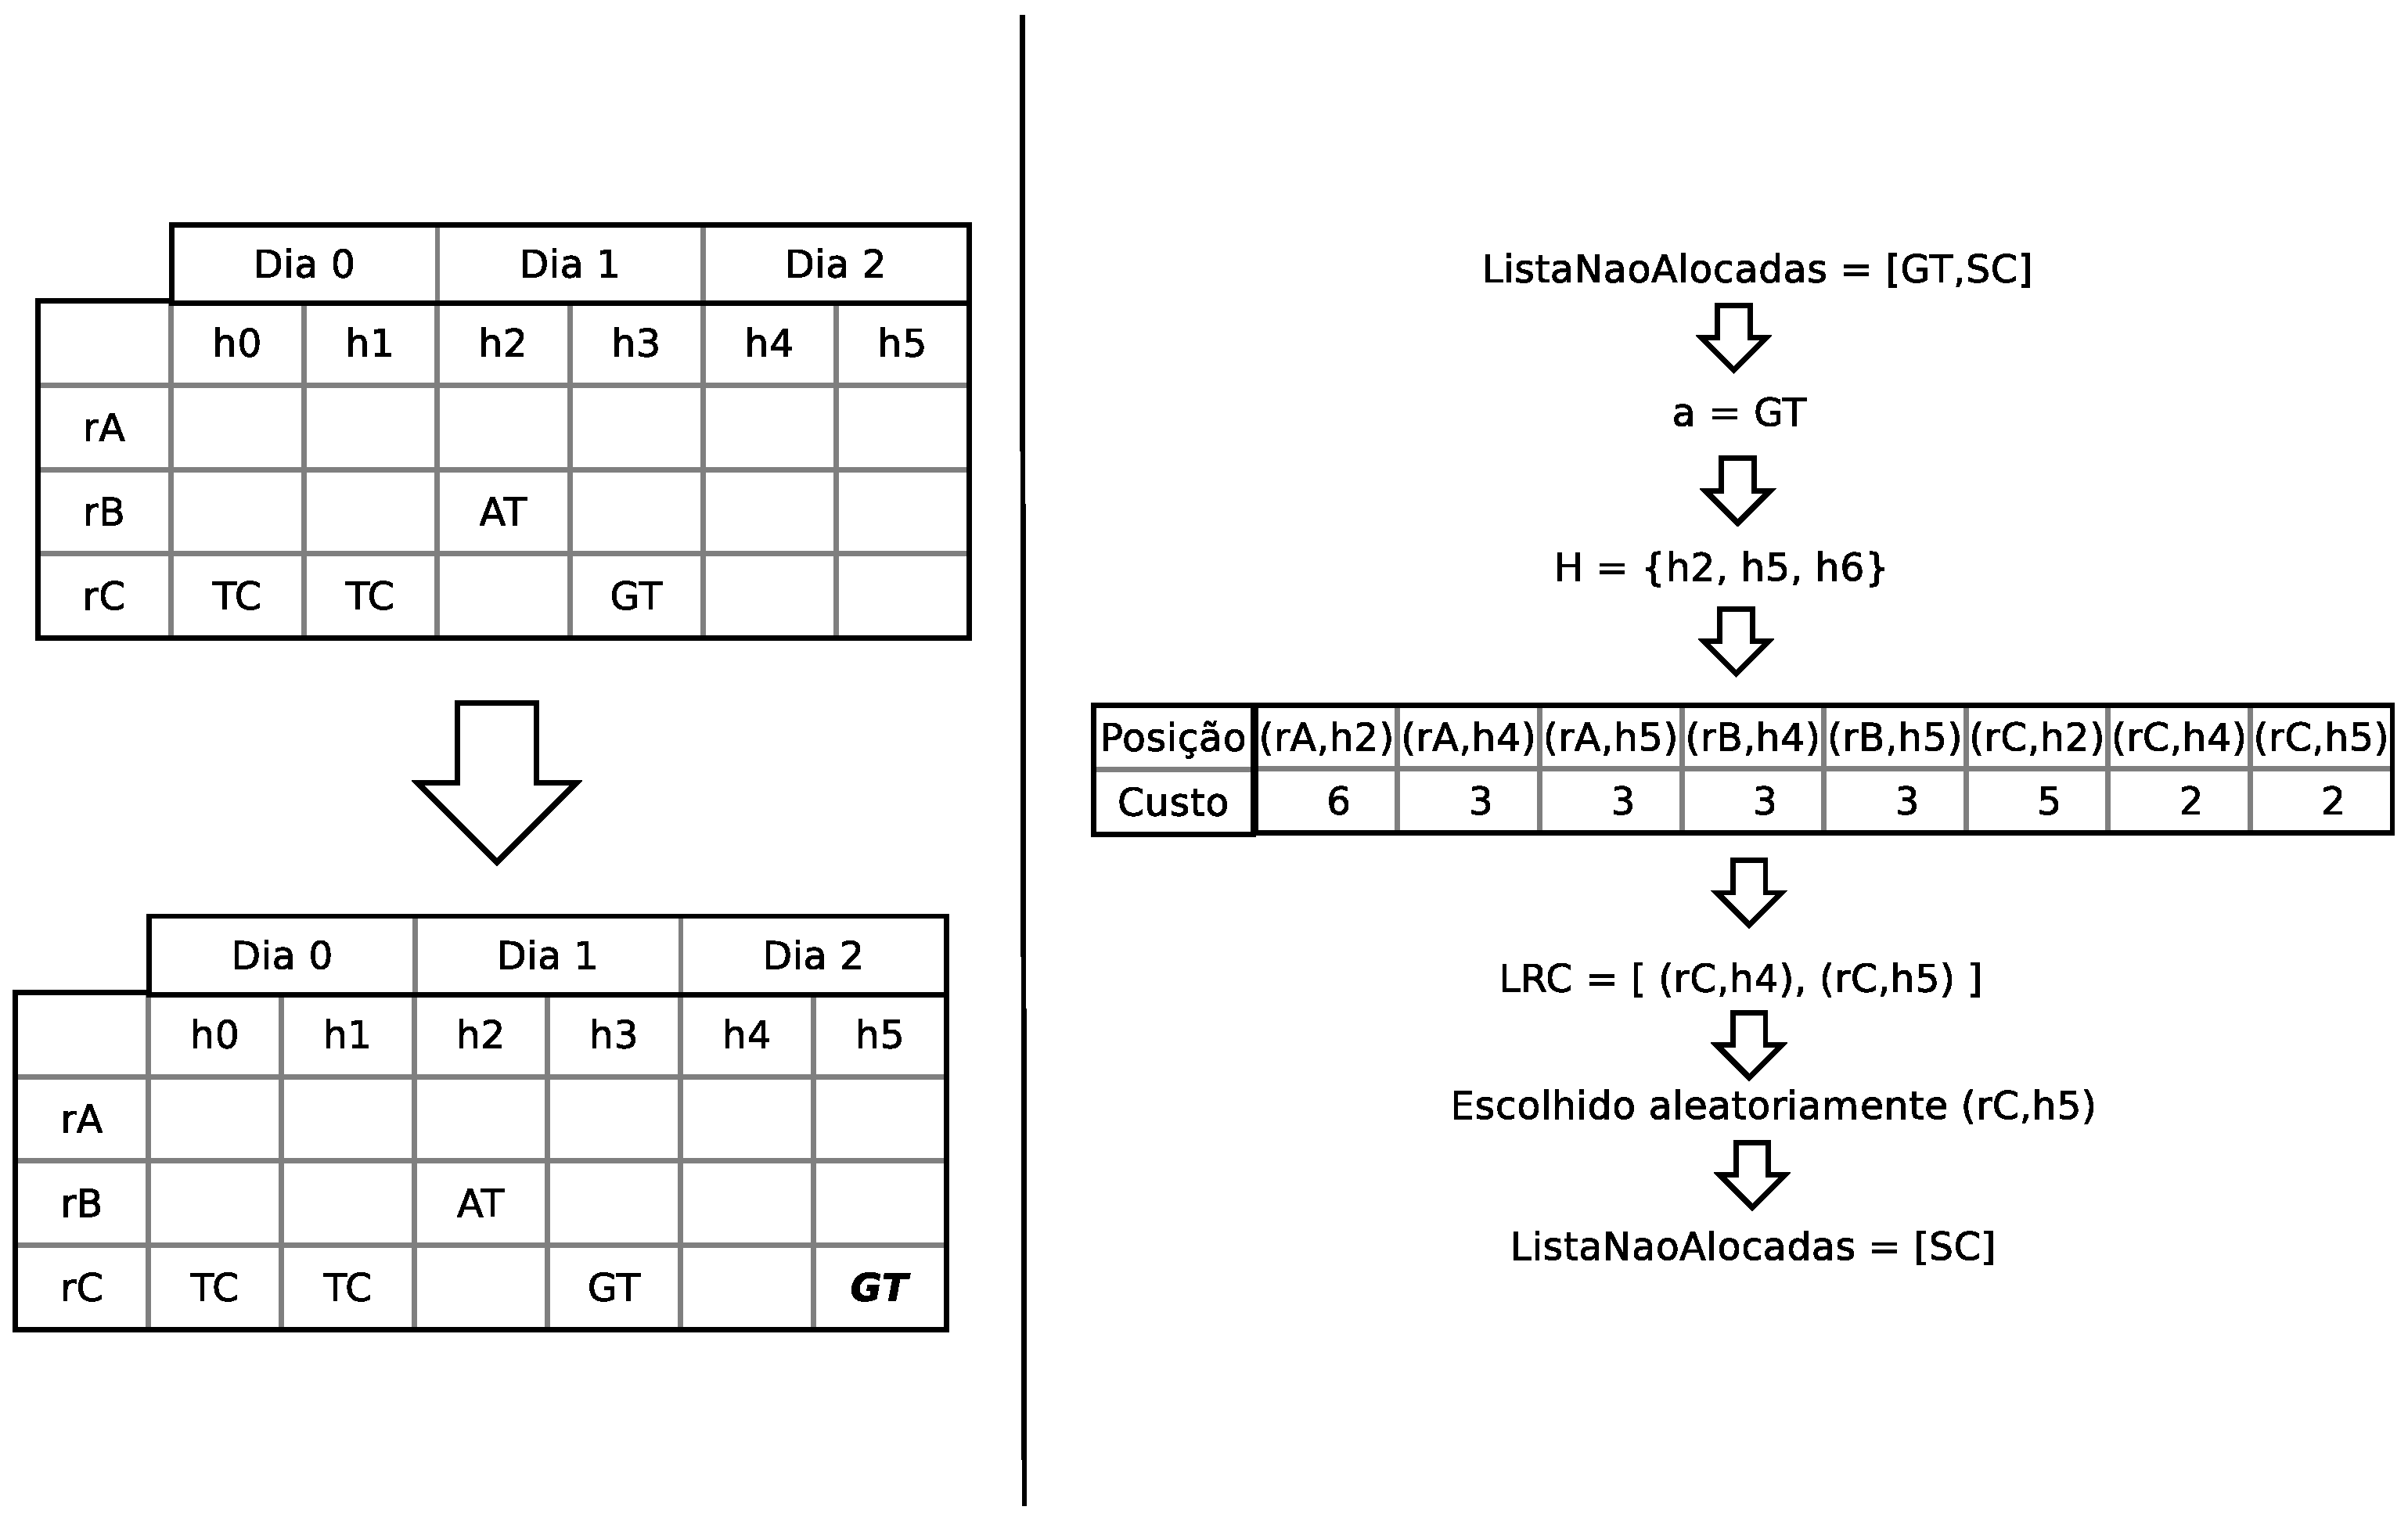
\includegraphics[width=15cm]{./SolInicial.eps}
 \caption[Etapa de construção de uma solução inicial]{Etapa de construção de uma solução inicial. À direita as etapas de uma iteração e à esquerda o antes e depois da tabela-horário.}
   \label{fig:solucao-inicial}
\end{center}
\end{figure}

As soluções produzidas pelo algoritmo \ref{solInicialGrasp-ITC2007} são sempre viáveis porque em cada iteração somente os horários que garantem a viabilidade são usados. No melhor caso o algoritmo termina após $n$ iterações, onde $n$ é a quantidade de aulas a serem alocadas. Quando há explosões, um número maior que $n$ iterações é executado porque aulas voltam para lista das não-alocadas. Experimentalmente foi verificado que também nestes casos o algoritmo converge e produz uma solução viável.

\subsection{Buscal local\label{subsec:abordagens}}

O objetivo da fase de busca local é melhorar a tabela-horário inicial. Para isso é preciso primeiro definir quais movimentos devem ser realizados para explorar a vizinhança da solução. Foram implementados dois movimentos distintos:

\begin{itemize}
\item \textbf{\textit{MOVE}}: Uma aula é movida para uma posição desocupada na tabela-horário.
\item \textbf{\textit{SWAP}}: Duas aulas trocam de posição na tabela-horário.
\end{itemize}

Como o GRASP não especifica qual estratégia de busca local, várias podem ser usadas. Neste trabalho fazemos uso de duas estratégias: a primeira, mais simples, do tipo \textit{Hill Climbing} e a segunda, \textit{Simulated Annealing}.

No \textit{Hill Climbing} \cite{Glover89}, a partir de uma solução inicial, em cada iteração um vizinho é gerado. Quando um vizinho com melhor valor de função objetivo é encontrado, ele passa a ser a solução atual. O algoritmo termina com $N$ iterações sem melhora da função objetivo, onde $N$ é parâmetro do algoritmo.

Particularmente para o ITC-2007, nos testes computacionais realizados, essa estratégia mos\-trou-se pouco eficiente, se prendendo facilmente em mínimos locais.

Uma modificação proposta foi trocar a busca em profundidade, tradicional no \textit{Hill Climbing}, por busca em largura. No entanto, a busca em largura é inviável para este problema, pois a quantidade de vizinhos de uma tabela-horário é muito grande. Assim, implementamos uma versão híbrida: em cada iteração são gerados $k$ vizinhos e, caso haja melhora, o melhor deles passa a ser a solução atual. Controlando o valor $k$ adequadamente esta versão consegue resultados superiores com uma eficiência compatível à busca em profundidade. Fazendo $k=1$, tem-se o algoritmo \textit{Hill Climbing} original.

\begin{algorithm}[H]
\label{algoHC}
\SetAlgoLined
\SetKwFunction{GeraSolucaoInicial}{GeraSolucaoInicial}
\SetKwFunction{BuscaLocal}{BuscaLocal}
\SetKwFunction{PathRelinking}{PathRelinking}
\SetKwFunction{AtualizaPool}{AtualizaPool}
\Entrada{Solução S , $N$, $k$}
\Saida{Melhor Solução $S^{*}$}

$i \leftarrow 0$ \;
$S^{*} \leftarrow S $ \;
\Enqto{$i < N$}{
	$S' \leftarrow GeraVizinho(S^{*}, k) $ \;
	$\Delta f \leftarrow f(S') - f(S^{*}) $ \;
	\Se{$ \Delta f < 0$}{
		$S^{*} \leftarrow S' $ \;
		$i = 0 $ \;
	}

	$i \leftarrow i + 1$ \;
}
\caption{\textit{Hill Climbing} com geração de k vizinhos por iteração}
\end{algorithm}

O algoritmo \ref{algoHC} mostra o algoritmo {\it Hill Climbing} modificado. Destaque para a função de geração de vizinho na linha 4. Além da solução atual, ela recebe como parâmetro o valor de $k$ que é a quantidade de vizinhos que serão gerados. A função retorna o melhor deles, $S'$. O algoritmo inicializa na linha um o contador de iterações sem melhora. Se o melhor vizinho gerado na linha 4 é melhor que a melhor solução encontrada ($\Delta f < 0$), então este vizinho passa a ser a solução atual e o contador de iterações sem melhora é zerado.

Foi verificado que esta nova versão consegue explorar melhor o espaço de soluções, conseguindo tabelas-horário melhores com menos tempo de execução.

Mas levando-se em conta os resultados conhecidos na literatura, as respostas não estavam satisfatórias para a maioria das instâncias. Foi necessário investir numa estratégia mais rebuscada, que intensifique bem a solução inicial e seja capaz de escapar de mínimos locais. A opção adotada foi usar \textit{Simulated Annealing} \cite{SA}. Essa estratégia de busca é inspirada num processo de metalurgia que aquece um material e resfria de modo controlado visando diminuir seus defeitos.

O algoritmo \textit{Simulated Annealing} (SA) possui três parâmetros principais: temperatura inicial, final e taxa de resfriamento. O algoritmo parte de uma temperatura inicial que vai sendo resfriada até chegar a temperatura final. Em cada temperatura, $N_v$ vizinhos são gerados. Se o vizinho gerado é melhor que a solução atual, esta é atualizada. Se o vizinho for pior, ele é aceito com uma probabilidade igual a $P = e^{-\Delta f/ T}$, onde $\Delta f$ é a diferença de valor da função objetivo do vizinho e da solução atual e $T$ é a temperatura atual. Quanto maior for $\Delta f$ e menor a temperatura, menores serão as chances de aceitar o vizinho. O comportamento típico do algoritmo é aceitar grande diversificação no início, quando a temperatura está alta. À medida que ela decresce, poucas pioras vão sendo aceitas e uma determinada região da busca é intensificada.

O algoritmo \ref{algoSA} apresenta o pseudo-código do \textit{Simulated Annealing} para o ITC-2007.

\begin{algorithm}[H]
\label{algoSA}
\SetAlgoLined
\SetKwFunction{GeraSolucaoInicial}{GeraSolucaoInicial}
\SetKwFunction{BuscaLocal}{BuscaLocal}
\SetKwFunction{PathRelinking}{PathRelinking}
\SetKwFunction{AtualizaPool}{AtualizaPool}
\Entrada{Solução S , $T_i$, $T_f$, $\beta$, $N_v$}
\Saida{Solução $S^{*}$}

$T \leftarrow T_i$ \;
$S^{*} \leftarrow S $ \;
\Enqto{$T > T_f$}{
	\Para{$i \leftarrow 1$ \Ate $N_v$}{
		$S' \leftarrow GeraVizinho(S^{*}) $ \;
		$\Delta f \leftarrow f(S') - f(S^{*}) $ \;
		\Se{$ \Delta f < 0$}{
			$S^{*} \leftarrow S' $ \;
		}\Senao{
			Gere um número aleatório $p \in (0, 1]$ \;
			\Se{$ p < e^{-\Delta f / T} $}{
				$S^{*} \leftarrow S' $ \;
			}
		}
	}
	$T \leftarrow T * \beta$
}
\caption{\textit{Simulated Annealing} para fase de busca local}
\end{algorithm}

Tanto no algoritmo \textit{Hill Climbing} quanto no \textit{Simulated Annealing}, a geração dos vizinhos é feita na mesma proporção de utilização dos movimentos: $50\%$ com \textit{MOVE} e $50\%$ com \textit{SWAP}. Em \cite{CDGS11b}, os mesmos movimentos são aplicados, mas para a segunda formulação do ITC-2007. Neste trabalho $60\%$ dos vizinhos são gerados com \textit{MOVE}, e os outros $40\%$ são gerados com \textit{MOVE} seguido de um \textit{SWAP}. Foi verificado através de testes que esta estratégia não se adapta tão bem à terceira formulação do campeonato. Gerando $50\%$ dos vizinhos com \textit{MOVE} e os outros $50\%$ somente com \textit{SWAP} o algoritmo atinge soluções melhores e de forma mais rápida. Uma possível explicação para este comportamento é que aplicando dois movimentos seguidos, um movimento pode interferir na melhora obtida pelo outro.

\subsection{Path-relinking}

No algoritmo proposto o \textit{Path-relinking} é aplicado sobre a solução obtida na busca local e uma solução do conjunto Elite. De acordo com \cite{Resende05graspwith}, o caminho percorrido entre as duas soluções pode ser feito de diversas maneiras. As duas principais são:

\begin{itemize}
\item \textbf{Religamento direto}: PR parte da solução pior em direção à melhor.
\item \textbf{Religamento inverso}: PR é aplicado partindo da melhor solução em direção à pior.
\end{itemize}

Pode se optar por construir os dois caminhos, com a desvantagem que o tempo de execução é o dobro. \cite{Resende05graspwith} indicam que no caso de fazer a opção por somente uma das trajetórias, as melhores soluções geralmente são encontradas utilizando religamento inverso. A explicação para isso é que boas soluções tendem a estar próximas à solução mais promissora. Sendo assim, o GRASP proposto neste trabalho aplica \textit{Path-relinking} usando uma solução elite como a inicial e a solução obtida na busca local é a solução alvo.

Durante a busca local, movimentos que introduzem inviabilidades na solução são descartados. Assim a viabilidade da solução obtida na fase de construção inicial fica garantida.

O algoritmo \ref{algoGraspFinal} resume a proposta desse trabalho: GRASP com PR para o problema de tabela-horário de universidades, terceira formulação do ITC-2007. Observe que a fase de busca local é configurável, podendo ser {\it Hill Climbing} ou {\it Simulated Annealing}, gerando duas versões diferentes.

\begin{algorithm}[H]
\label{algoGraspFinal}
\SetAlgoLined
\SetKwFunction{GeraSolucaoInicial}{GeraSolucaoInicial}
\SetKwFunction{BuscaLocal}{BuscaLocal}
\SetKwFunction{PathRelinking}{PathRelinking}
\SetKwFunction{AtualizaPool}{AtualizaPool}
\Entrada{MaxIter, MaxElite}
\Saida{Melhor Solução $S^{*}$}

$f^{*} \leftarrow \infty $ \;
$Elite \leftarrow \emptyset $ \;
\Para{$i\leftarrow 1$ \Ate $MaxIter$}{
	$S \leftarrow GeraSolucaoInicial() $ \;
	$S \leftarrow BuscaLocal(S) $  \tcp{Hill Climbing ou Simulated Annealing} 
	\Se{$ i \geq 2 $}{
		Selecione aleatoriamente $S_{elite} \in Elite $ \;
		$S \leftarrow PathRelinking(S, S_{elite}) $ \;
	}
	\Se{$ f(S) < f^{*} $}{
		$S^{*} \leftarrow S $ \;
		$f^{*} \leftarrow f(S) $ \;
	}
	$AtualizaElite(S, Elite) $ \;
}
\caption{Algoritmo GRASP para o ITC-2007}

\end{algorithm}


\chapter{Resultados Computacionais\label{cap:resultados}}

%\vfill{}
%\begin{flushright}{}``\emph{Nada se cria, nada se perde, tudo se transforma.}''\\
%{\small Lavousier}\end{flushright}{\small \par}
%\vfill{}

Neste capítulo são apresentados alguns detalhes de implementação não mencionados no capítulo anterior. Também são descritas as instâncias usadas para testar os algoritmos e mencionado como foram feitas as escolhas dos parâmetros do GRASP, além dos parâmetros específicos das buscas locais \textit{Hill Climbing} e \textit{Simulated Annealing}. No final do capítulo os resultados obtidos pelos algoritmos são tabulados e comparados com os resultados oficiais do ITC-2007.
%\newpage

\section{Descrição das instâncias utilizadas}

As instâncias utilizadas foram as mesmas submetidas aos competidores do ITC-2007.
São 21 instâncias ao todo, com grau de dificuldade variado. A organização garante que existe solução viável para todas as instâncias, fato que foi comprovado nos testes. Mas nada foi informado sobre a quantidade de violações fracas em cada instância. Em \cite{itc2007} podem ser obtidas todas as instâncias.

Na tabela \ref{tab:instancias} são apresentados os dados mais relevantes de cada instância. A quantidade de horários de aula numa semana não varia muito de instância para instância. A coluna conflitos conta a quantidade de pares de aula que não podem ser alocadas no mesmo horário (mesma disciplina, mesmo currículo ou mesmo professor) dividido pelo total de pares distintos de aula. A disponibilidade mede percentualmente a quantidade de horários que são disponíveis para as aulas, levando-se em consideração as restrições de indisponibilidade que são informadas no arquivo de entrada.

A quantidade de currículos e disciplinas tem grande impacto no tempo de execução do algoritmo, pois são mais aulas para fazer a contagem total de violações. A quantidade de conflitos e disponibilidade influencia na dificuldade de encontrar uma solução viável, pois quanto mais conflitos e menos disponibilidade, menos horários existirão para alocar aula sem violar as restrições fortes. Além de dificultar a viabilidade no momento de geração da solução inicial, os conflitos e as disponibilidades dificultam a exploração da vizinhança na busca local, dado que muitas trocas acabam sendo descartadas por introduzirem violações das restrições fortes.

\begin{center}
\begin{table}[!htb]
\begin{tabular}{|c|c|c|c|c|c|c|c|}\hline
{\bf Instância} & {\bf Currículos} & {\bf Salas} & {\bf Disciplinas} &{\bf Horários}&{\bf Dias}&{\bf Conflitos} & {\bf Disponibi-}\\
 &  &  &  &{\bf por dia} & & & {\bf lidade} \\\hline
comp01 & 14 & 6 & 30 & 6 & 5 & 13.2 & 93.1 \\ 
comp02 & 70 & 16 & 82 & 5 & 5 & 7.97 & 76.9 \\ 
comp03 & 68 & 16 & 72 & 5 & 5 & 8.17 & 78.4 \\ 
comp04 & 57 & 18 & 79 & 5 & 5 & 5.42 & 81.9 \\ 
comp05 & 139 & 9 & 54 & 6 & 6 & 21.7 & 59.6 \\ 
comp06 & 70 & 18 & 108 & 5 & 5 & 5.24 & 78.3 \\ 
comp07 & 77 & 20 & 131 & 5 & 5 & 4.48 & 80.8 \\ 
comp08 & 61 & 18 & 86 & 5 & 5 & 4.52 & 81.7 \\ 
comp09 & 75 & 18 & 76 & 5 & 5 & 6.64 & 81 \\ 
comp10 & 67 & 18 & 115 & 5 & 5 & 5.3 & 77.4 \\ 
comp11 & 13 & 5 & 30 & 9 & 5 & 13.8 & 94.2 \\ 
comp12 & 150 & 11 & 88 & 6 & 6 & 13.9 & 57 \\ 
comp13 & 66 & 19 & 82 & 5 & 5 & 5.16 & 79.6 \\ 
comp14 & 60 & 17 & 85 & 5 & 5 & 6.87 & 75 \\ 
comp15 & 68 & 16 & 72 & 5 & 5 & 8.17 & 78.4 \\ 
comp16 & 71 & 20 & 108 & 5 & 5 & 5.12 & 81.5 \\ 
comp17 & 70 & 17 & 99 & 5 & 5 & 5.49 & 79.2 \\ 
comp18 & 52 & 9 & 47 & 6 & 6 & 13.3 & 64.6 \\ 
comp19 & 66 & 16 & 74 & 5 & 5 & 7.45 & 76.4 \\ 
comp20 & 78 & 19 & 121 & 5 & 5 & 5.06 & 78.7 \\ 
comp21 & 78 & 18 & 94 & 5 & 5 & 6.09 & 82.4 \\
\hline
\end{tabular}
\caption{Tabela com informações sobre cada instância do ITC-2007}
\label{tab:instancias}
\end{table}
\end{center}

\section{Detalhes de implementação\label{sec:detalhes-implementacao}}

Todas as implementações foram feitas na linguagem C. A tabela-horário é representada com uma matriz, onde as linhas representam as salas e as colunas representam os horários de todos os dias. As aulas são representadas por números inteiros. Cada aula da disciplina é representada por um número diferente. Se a primeira disciplina da instância possui cinco aulas semanais, então elas são representadas com os números 1, 2, 3, 4 e 5. Uma segunda disciplina com três aulas é representada na tabela com os números 6, 7 e 8, e assim por diante. Horários vagos são representados com o valor $-1$.

A tabela \ref{tab:solucao_toy_codificada} é a mesma representação da tabela-horário \ref{tab:solucao_toy} usando a codificação com números inteiros. São três aulas para \textit{SecCosC}, três para \textit{ArcTec}, cinco para \textit{TecCos} e cinco para \textit{Geotec}, totalizando 16 aulas que estão destacadas em negrito. Todas as demais são horários desocupados.

\begin{center}
\begin{table}[!htb]
%\begin{footnotesize}
{\fontsize{9}{12} \selectfont
\begin{tabular}{|c|c|c|c|c||c|c|c|c||c|c|c|c||c|c|c|c||c|c|c|c|}\hline
 & \multicolumn{4}{|c||}{Dia 0} & \multicolumn{4}{|c||}{Dia 1}& \multicolumn{4}{|c||}{Dia 2}& \multicolumn{4}{|c||}{Dia 3}&  \multicolumn{4}{|c|}{Dia 4}\\ \hline
 & 0 & 1 & 2 & 3 & 0 & 1 & 2 & 3 & 0 & 1 & 2 & 3 & 0 & 1 & 2 & 3 & 0 & 1 & 2 & 3 \\ \hline
rA & -1 & {\bf 12} & -1 & -1 & {\bf 13} & -1 & {\bf 14} & {\bf 15} & -1 & -1 & -1 & -1 & -1 & -1 & -1 & -1 & -1 & -1 & -1 & {\bf 16} \\ \hline
rB & -1 & -1 & {\bf 4} & -1 & {\bf 5} & -1 & -1 & -1 & -1 & -1 & -1 & -1 & -1 & -1 & -1 & -1 & -1 & -1 & -1 & -1 \\ \hline
rC & -1 & {\bf 7} & -1 & -1 & -1 & {\bf 8} & {\bf 1} & -1 & -1 & -1 & {\bf 2} & {\bf 9} & {\bf 3} & -1 & -1 & -1 & {\bf 10} & -1 & {\bf 11} & {\bf 6} \\ \hline
\end{tabular}
}
%\end{footnotesize}
\caption{Tabela-horário para a instância \textit{Toy} codificando as aulas com números inteiros}
\label{tab:solucao_toy_codificada}
\end{table}
\end{center}

Algumas matrizes auxiliares foram utilizadas para extrair informações de forma mais rápida. Algumas delas são estáticas pois dependem apenas das informações presentes no arquivo de entrada. Outras são dinâmicas para refletir o estado atual da tabela-horário que está sendo considerada.

Descrevemos, a seguir, as duas matrizes estáticas. Considere $N$ o número total de aulas na instância e $H$ o total de horários, que é a quantidade de dias multiplicada pela quantidade de períodos de aula em um dia.

A primeira matriz, chamada de $AA$, possui dimensão $N \times N$. Ela é utilizada para descobrir de forma rápida se duas aulas têm conflito entre si, ou se pertencem a mesma disciplina. Dadas duas aulas $a_1$ e $a_2$, adota-se a seguinte convenção:

\begin{itemize}
\item $AA[a_1][a_2] = 2$: as duas aulas são da mesma disciplina;
\item $AA[a_1][a_2] = 1$: as duas aulas possuem conflitos entre si, seja por estarem num mesmo currículo ou por serem lecionadas pelo mesmo professor;
\item $AA[a_1][a_2] = 0$: não há conflitos entre as aulas e elas não pertencem a mesma disciplina.
\end{itemize}

A segunda matriz estática, chamada de $AI$, possui dimensão $N \times H$. Ela é utilizada para verificar quais horários são disponíveis para as aulas segundo as restrições de indisponibilidade que são informadas no arquivo de entrada. Dois valores são possíveis nesta matriz:

\begin{itemize}
\item $AI[a][h] = 1$: a aula $a$ é indisponível no horário $h$;
\item $AI[a][h] = 0$: a aula $a$ pode ser alocada no horário $h$.
\end{itemize}

É preciso ressaltar que somente $AI[a][h] = 0$ não garante a possibilidade de $a$ ser alocada no horário $h$. Durante a execução do algoritmo é necessário avaliar a tabela-horário em questão para saber se existe alguma sala desocupada no horário $h$ e/ou se nenhuma aula já alocada no horário é conflitante com $a$.

As matrizes dinâmicas refletem o estado da tabela-horário que está sendo considerada. O objetivo principal destas tabelas é fazer a contagem das violações fracas de forma mais eficiente. Considere $C$ o total de currículos, $DC$ o total de disciplinas, $D$ a quantidade de dias, $P$ a quantidade de períodos de aula em um dia e $S$ o total de salas.

A primeira matriz é $DiscDias$ com dimensão $DC \times D$. Para uma dada disciplina $disc$ e um dia $d$, $DiscDias[disc][dia]$ retorna a quantidade de aulas da disciplina $disc$ no dia $d$. Com esta matriz é possível contar mais rapidamente em quantos dias há aulas de uma certa disciplina, facilitando o cálculo da contagem das violações de dias mínimos de trabalho.

A segunda matriz, $DiscSalas$, tem dimensão $DC \times S$. Para uma dada disciplina $disc$ e uma sala $s$, $DiscSalas[disc][s]$ retorna a quantidade de aulas da disciplina $disc$ na sala $s$ durante a semana. Analogamente esta matriz tem por objetivo verificar quantas salas estão sendo ocupadas pela disciplina, facilitando a contagem das violações referentes à estabilidade de sala.

A terceira matriz, $CurrDiasPeriodos$, é tridimensional com tamanho $C \times D \times P$. Dados um currículo $c$, um dia $d$ e um período $p$, $CurrDiasPeriodos[c][d][p]$ retorna a quantidade de aulas do currículo $c$ alocadas no dia $d$ e horário $p$. Esta matriz é usada para verificar se um currículo está com aulas isoladas. Se um currículo $c$ possui alguma aula no dia $d$ e horário $p$, mas $CurrDiasPeriodos[c][d][p-1] = 0$ e $CurrDiasPeriodos[c][d][p+1] = 0$ então o currículo $c$ não tem nenhuma aula no período anterior nem no próximo, o que gera uma violação de aulas isoladas.

As matrizes dinâmicas são atualizadas quando um novo vizinho é gerado. Supondo que a aula $a$ da disciplina $disc$ foi movida da posição $(s1, d1, p1)$ para a posição $(s2, d2, p2)$  e que $disc$ pertence ao conjunto de currículos $C_a$ (pode ser mais de um currículo), as seguintes operações serão feitas:

\begin{equation}
\begin{split}
DiscDias[disc][d1] = DiscDias[disc][d1] - 1 \\
DiscDias[disc][d2] = DiscDias[disc][d2] + 1 \\
DiscSalas[disc][s1] = DiscSalas[disc][s1] - 1 \\
DiscSalas[disc][s2] = DiscSalas[disc][s2] + 1 \\
CurrDiasPeriodos[c][d1][p1] = CurrDiasPeriodos[c][d1][p1] - 1, \forall c \in C_a \\
CurrDiasPeriodos[c][d2][p2] = CurrDiasPeriodos[c][d2][p2] + 1, \forall c \in C_a \\
\end{split}
\end{equation}

Além das matrizes auxiliares, outro detalhe importante é a geração e avaliação dos vizinhos. Num primeiro momento, para avaliar um vizinho gerado, o movimento era aplicado e a função objetivo avaliava toda a tabela-horário. Dado que \textit{MOVE} e \textit{SWAP} alteram apenas duas posições, é mais eficiente verificar o efeito das trocas localmente já que o restante da tabela permanece inalterado. Assim, as funções de geração de vizinhos retornam, além das posições de troca, um valor $\Delta f$. Se $\Delta f$ é menor que zero, então significa que o vizinho terá um melhor valor de função objetivo.

Na figura \ref{fig:diagramaDeClasses} podem ser vistas as estruturas de dados usadas no trabalho. Todas elas correspondem a um {\it struct} no código-fonte. O {\it struct} \texttt{Problema} contém as informações básicas, como quantidade de dias, períodos e salas, e ainda pendura as listas de currículos, disciplinas, salas e restrições de indisponibilidade. Ela também armazena as matrizes estáticas que não variam durante a execução do algoritmo.

A tabela-horário é representada pelo {\it struct} \texttt{Tabela}. Ela possui uma matriz que segue a representação da tabela \ref{tab:solucao_toy_codificada}, além de armazenar o valor da função objetivo e as matrizes dinâmicas.

\begin{figure}[!htb]
\begin{center}
  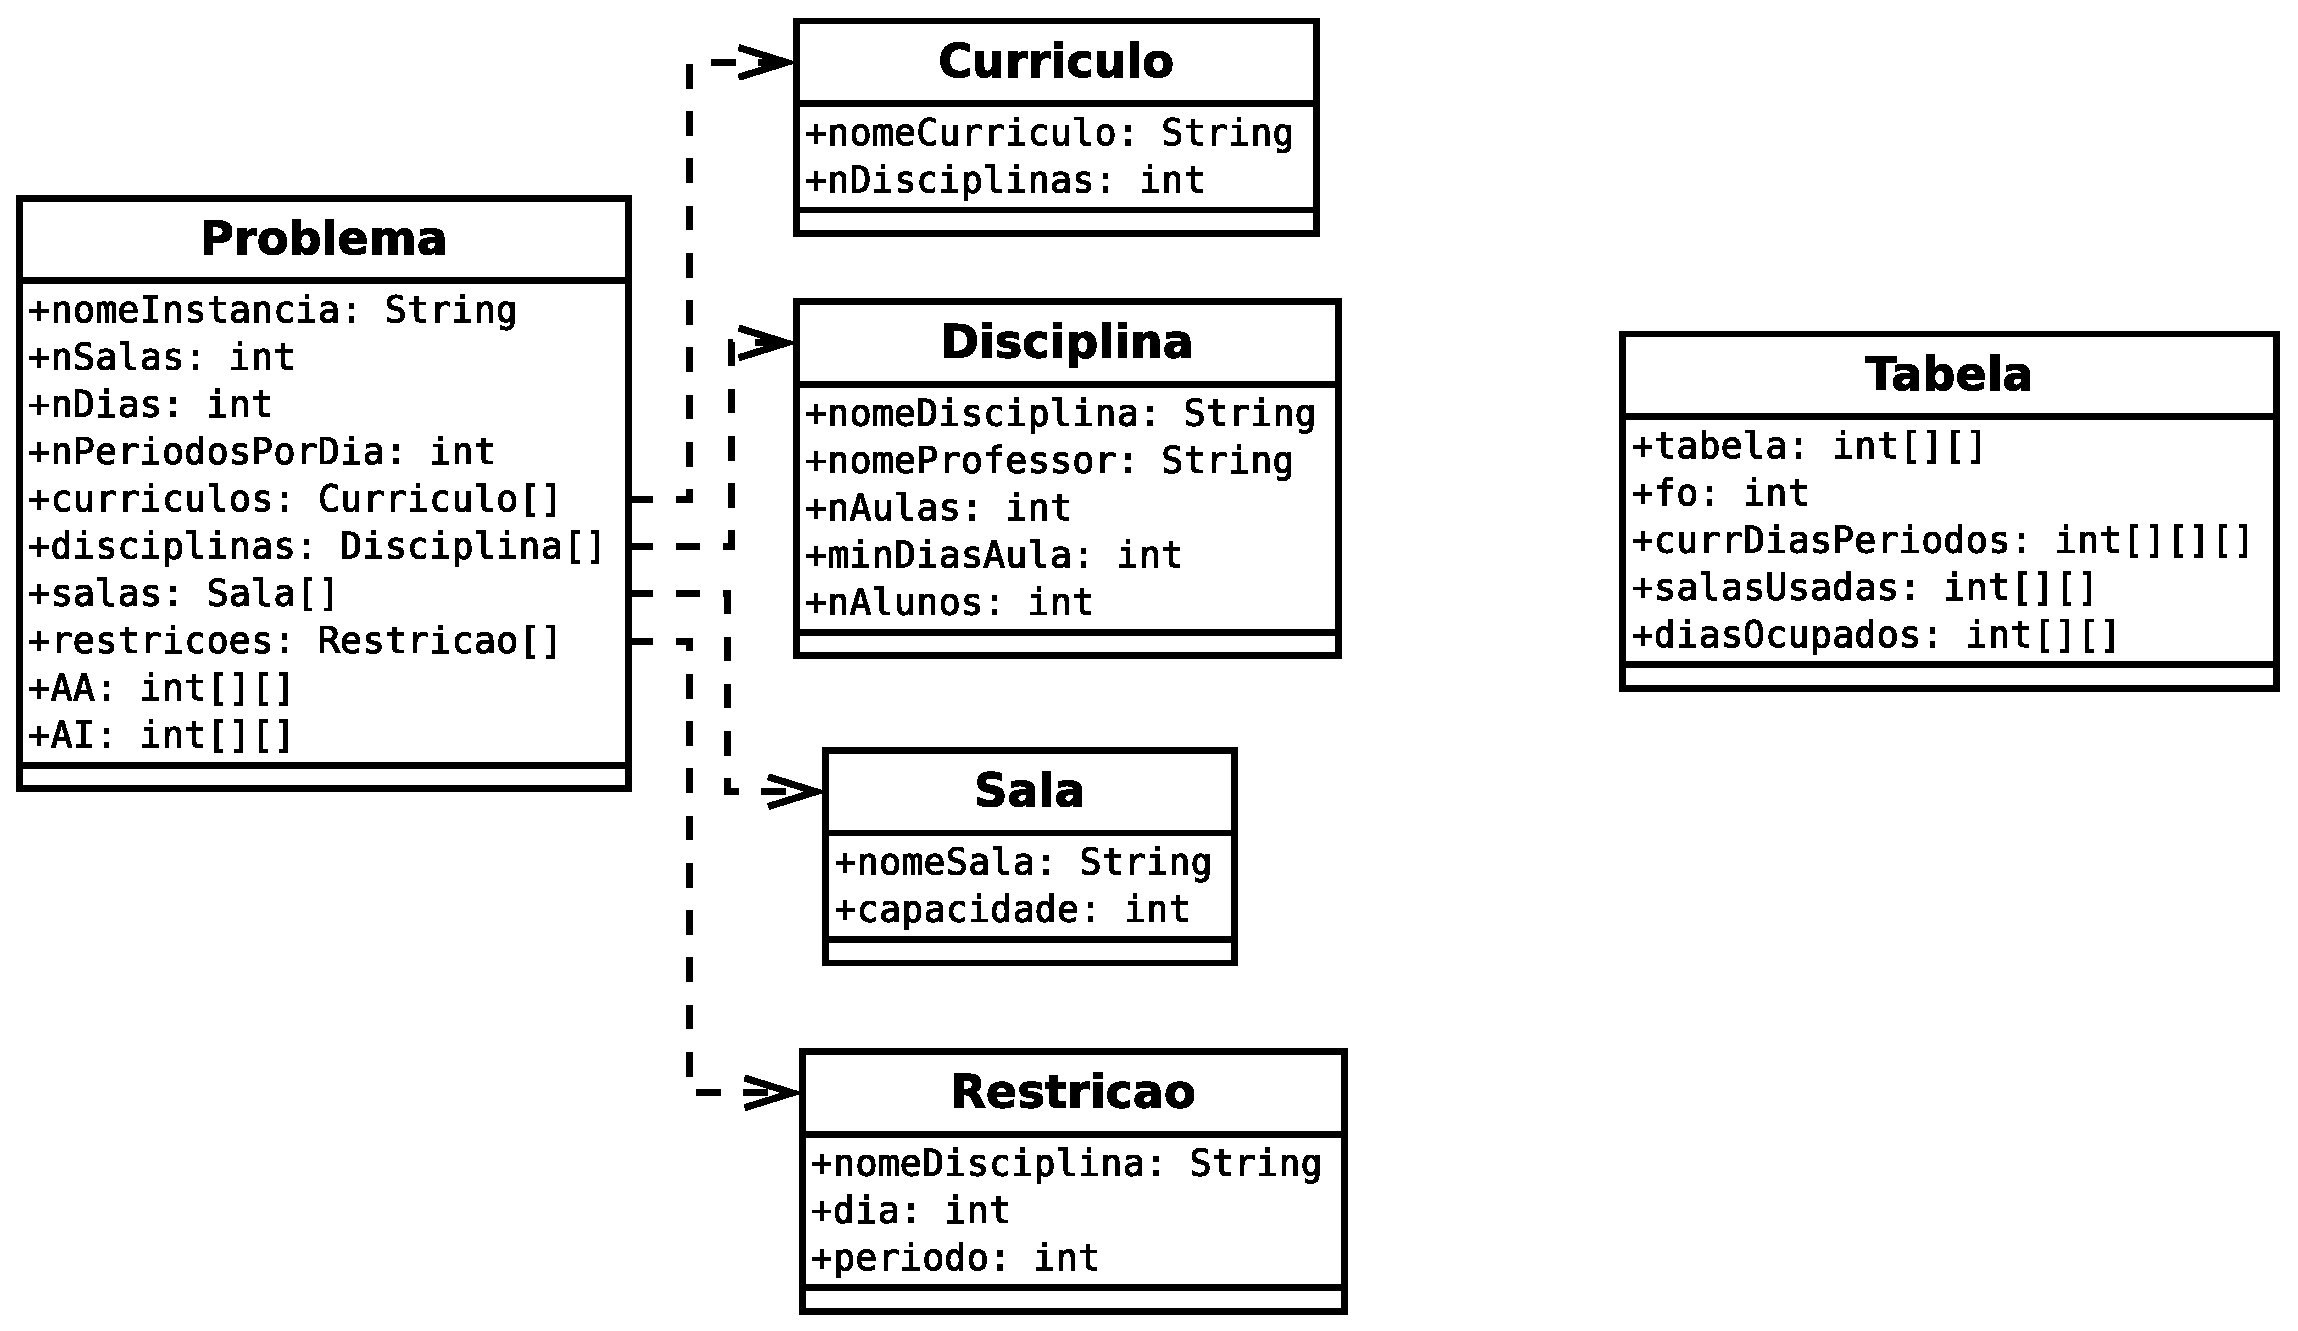
\includegraphics[width=14cm]{./Diagrama.eps}
 \caption{Diagrama de classes das estruturas para modelagem da instância e da tabela-horário}
   \label{fig:diagramaDeClasses}
\end{center}
\end{figure}


\section{Escolha dos parâmetros}

O algoritmo GRASP possui dois parâmetros: número máximo de iterações \textit{MaxIter} e o valor $\alpha$ que regula a forma de construção da solução inicial. Como foi implementado \textit{Path-relinking}, um terceiro parâmetro, \textit{MaxElite}, foi adicionado para limitar o tamanho do conjunto de soluções elite.

Quanto mais iterações, mais soluções o algoritmo pode explorar. Foi escolhido limitar a quantidade de iterações em 200. Mas como o campeonato exige que o algoritmo execute em aproximadamente 10 minutos, não é possível executar essa quantidade de iterações. O número máximo de soluções elite foi fixado em 20.

O parâmetro $\alpha \in [0, 1]$ é mais delicado. Se o seu valor for muito próximo de 0, o algoritmo de construção inicial tem comportamento mais guloso, produzindo soluções de boa qualidade porém pouco diversificadas. Se $\alpha$ é mais próximo de 1, as soluções são mais diversificadas mas com a desvantagem que elas tem um valor alto de função objetivo. Foram testados diversos valores no intervalo $[0.01, 0.5]$. Foi comprovado que quanto menor o valor de $\alpha$, melhor a qualidade da solução, mas ainda longe do que é possível alcançar com a busca local. Foi decidido usar $\alpha = 0.15$, por produzir alguma diversificação nas soluções iniciais e manter uma qualidade razoável.

Os demais parâmetros são específicos das buscas locais. O algoritmo \textit{Hill Climbing} possui o parâmetro $N$, que limita a quantidade máxima de iterações sem melhora na função objetivo. Um valor grande de $N$ permite maior exploração dos vizinhos, mas consome maior tempo de execução. Como a idéia do GRASP é explorar soluções diferentes, $N$ foi fixado em 10000, a partir de testes preliminares. Empiricamente esse valor permite explorar bem a solução inicial sem perder muito tempo em um mínimo local. Um segundo parâmetro introduzido no algoritmo foi $k$, que fornece a quantidade de vizinhos que serão gerados por iteração. Através de testes preliminares, verificamos que com valor de $k=10$, o algoritmo produz boas soluções e mantém um desempenho compatível com a versão original, isto é, $k=1$ (apenas um vizinho). Valores maiores de $k$ tornam o algoritmo lento e não há ganho justificável na qualidade das soluções.

O algoritmo \textit{Simulated Annealing} possui mais parâmetros, tornando a tarefa de calibração mais difícil. Foram escolhidos parâmetros que permitem um certo grau de diversificação no início da busca e maior intensificação no final do processo. Como o algoritmo de solução inicial já fornece uma resposta com qualidade razoável, a temperatura inicial não precisa ser muito alta. Foi observado nos testes preliminares que fixar temperaturas altas com uma solução inicial de boa qualidade não ajuda muito o processo, pois permite aceitar soluções muito ruins e a melhora é observada apenas quando o resfriamento está bem adiantado. Foi observado também que, particularmente para as instâncias do ITC-2007, quando o algoritmo atinge uma temperatura abaixo de $0,01$ a busca estabiliza e raramente uma solução melhor é encontrada.

Com base nestas observações foram escolhidos os seguintes parâmetros: $T_i = 1,5$, $T_f = 0,005$, $\beta = 0,999$. Um valor de $\beta$ um pouco maior poderia ser utilizado para fazer um resfriamento mais lento e explorar mais o espaço de busca, mas devido ao limitante de tempo estipulado pelo ITC-2007, o valor de $\beta$ foi fixado em $0,999$. Em cada temperatura são gerados $N_v = 500$ vizinhos.

Uma boa ferramenta que auxilia a calibração de parâmetros de algoritmos como o \textit{Simulated Annealing} é o pacote \textit{irace} da linguagem \textit{R} \cite{irace}. Ele permite explorar de forma mais eficiente as combinações de parâmetros, reduzindo o esforço necessário para esta terefa. Neste trabalho ele só foi usado em testes iniciais do SA sem o GRASP.

Como explicado na subseção \ref{subsec:abordagens}, os vizinhos em todas as buscas locais são gerados somente com \textit{MOVE} ou somente com \textit{SWAP}. Os dois movimentos têm igual probabilidade de ocorrer.

O algoritmo {\it Path-relinking} implementado não possui parâmetros. A única decisão a tomar está relacionada a forma de ligar duas soluções. Testes confirmaram que as observações de \cite{Resende05graspwith} se aplicam ao problema em questão, e o religamento inverso é superior ao direto. Sendo assim, o algoritmo parte de uma solução elite em direção a uma solução ótima local.

Todas estas escolhas de parâmetros foram feitas usando um subconjunto das 21 instâncias, procurando observar o comportamento dos algoritmos com exemplares classificados, quanto ao número de conflitos, em fáceis, intermediários e difíceis. As instâncias escolhidas foram respectivamente \textit{comp01}, \textit{comp17} e \textit{comp05}.

\section{Análise dos resultados}

Todos os algoritmos descritos neste trabalho foram implementados na linguagem C, compilados com GCC 4.1.2 e testados em máquina Linux com a distribuição Fedora Core 8, com processador Intel quad-core 2.4 GHz e 2 Gb de memória RAM.

Os organizadores do campeonato forneceram um programa executável para fazer um \textit{benchmark} na máquina de testes dos competidores. O objetivo desse programa é informar um tempo de execução que seria equivalente nas máquinas do campeonato. Utilizando esse programa na máquina onde os testes foram realizados, foi estipulado um tempo de execução de 324 segundos.

Foi necessário adicionar nos algoritmos o critério de parada pelo tempo de execução, pois nos algoritmos apresentados nesse trabalho, o único critério considerado foi número máximo de iterações {\it{MaxIter}}.

Uma das melhorias implementadas no algortimo, que foi citada na seção \ref{sec:detalhes-implementacao}, é a geração e avaliação dos vizinhos de uma solução. Com o intuito de medir a eficiência desta modificação descrita foram criados dois programas para gerar uma tabela-horário inicial aleatória e, em seguida, gerar e avaliar 100000 vizinhos desta tabela. No primeiro programa a avaliação é feita levando em consideração toda a tabela. No segundo a avaliação é apenas local. Usando a instância \textit{comp01} como parâmetro e executando cada programa três vezes, o primeiro executou as 100000 avaliações em um tempo computacional em torno de $44.996$ segundos na média, enquanto o segundo programa executou em torno de $4.242$ segundos na média. O \textit{speedup} aproximado foi portanto de 10 vezes. Utilizando a instância \textit{comp12}, que é uma instância maior, o primeiro programa executou em torno de $467.603$ segundos na média, enquanto o segundo em $19.803$ segundos. Nesta instância o \textit{speedup} foi superior a 23 vezes. Observem que o ganho de eficiência foi bem significativo para a instância maior.

O algoritmo GRASP proposto foi executado para as 21 instâncias do ITC-2007. Para avaliar a eficiência dos tipos de busca local abordadas nesse trabalho, três versões do algoritmo foram testadas:

\begin{itemize}
\item {\bf GHC1}: Busca local {\it{Hill Climbing}} com $k=1$ (Somente um vizinho é gerado por iteração).
\item {\bf GHC2}: Busca local {\it{Hill Climbing}} com $k=10$ (10 vizinhos são gerados por iteração).
\item {\bf GSA}: Busca local {\it{Simulated Annealing}}, com $T_i = 1,5, T_f = 0,005, \beta = 0,999, N_v = 500$.
\end{itemize}

Tanto em GHC1 quanto em GHC2 a quantidade máxima de iterações sem melhora é fixada em $N = 10000$.

A tabela \ref{tab:resultados_gerais} lista as melhores respostas encontradas para cada instância do ITC-2007. Os valores informados se referem apenas às violações das restrições fracas, dado que todas as soluções são viáveis. Assim como foi feito no ITC-2007, cada algoritmo foi executado 10 vezes com diferentes \textit{seeds} para geração de números aleatórios. Todas as execuções foram limitadas em 324 segundos.


\begin{table}[htbf]
\begin{center}
\begin{tabular}{|l|c|c|c|}
\hline
Instância & GHC1 & GHC2 & GSA \\ \hline
comp01	& 15	& {\bf 5}	& {\bf 5} \\
comp02	& 260	& 130	& {\bf 73} \\
comp03	& 223	& 125	& {\bf 98} \\
comp04	& 168	& 73	& {\bf 48} \\
comp05	& 707	& 525	& {\bf 409} \\
comp06	& 293	& 116	& {\bf 75} \\
comp07	& 266	& 68	& {\bf 36} \\
comp08	& 186	& 77	& {\bf 58} \\
comp09	& 269	& 144	& {\bf 119} \\
comp10	& 245	& 68	& {\bf 41} \\
comp11	& 9	& {\bf 0}	& {\bf 0} \\ \hline
\end{tabular}
\medskip
\begin{tabular}{|l|c|c|c|}
\hline
Instância & GHC1 & GHC2 & GSA \\ \hline
comp12	& 847	& 455	& {\bf 375} \\
comp13	& 206	& 110	& {\bf 97} \\
comp14	& 191	& 91	& {\bf 72} \\
comp15	& 218	& 141	& {\bf 101} \\
comp16	& 233	& 96	& {\bf 69} \\
comp17	& 271	& 127	& {\bf 105} \\
comp18	& 179	& 113	& {\bf 102} \\
comp19	& 238	& 122	& {\bf 87} \\
comp20	& 356	& 106	& {\bf 88} \\
comp21	& 301	& 176	& {\bf 136} \\ \hline
Média & 270,52  & 136,57 & {\bf 104,47}  \\ \hline
\end{tabular}
\caption{Melhores respostas obtidas pelas três versões do algoritmo: GHC1, GHC2 e GSA}
\label{tab:resultados_gerais}
\end{center}
\end{table}


Na tabela \ref{tab:resultados_gerais} pode ser observado que o algoritmo GSA é o melhor dentre as três versões descritas, sendo superior em 19 instâncias e empatando com GHC2 nas instâncias \textit{comp01} e \textit{comp11}. Na média, GSA supera GHC1 em $258\%$ e GHC2 em $30\%$.

Nas tabelas \ref{tab:solucoes_itc2007_1} e \ref{tab:solucoes_itc2007_2} podem ser vistos os resultados obtidos pelos competidores. As colunas estão ordenadas pelas médias das respostas obtidas. Em cada tabela foi adicionada uma coluna com os resultados obtidos pelo melhor algoritmo implementado neste trabalho, o GSA. A melhor resposta de cada instância está destacada em negrito.

A competição foi dividida em duas fases descritas a seguir. A primeira fase foi mais geral e durou aproximadamente 6 meses. Todos os competidores registrados receberam sete instâncias inicialmente e mais sete faltando duas semanas para o encerramento da fase. Eles submeteram os algoritmos e as melhores respostas encontradas para cada instância. A tabela \ref{tab:solucoes_itc2007_1} lista os resultados desta primeira fase.

Os cinco melhores algoritmos da fase inicial (finalistas) foram selecionados para a segunda fase. Nesta segunda etapa os organizadores executaram os cinco melhores algoritmos com mais sete instâncias chamadas de ocultas por não serem conhecidas previamente pelos competidores. A tabela \ref{tab:solucoes_itc2007_2} lista os resultados dos finalistas com estas instâncias. Os resultados da primeira fase foram obtidos sem direitos de publicação dos nomes dos não-finalistas, por isso estão identificados apenas como 6º lugar, 7º lugar e assim por diante. Os cinco finalistas na ordem de classificação são:

\begin{enumerate}
\item Tomas Müller (Estados Unidos)
\item Zhipeng Lu e Jin-Kao Hao (França)
\item Mitsunori Atsuta, Koji Nonobe, e Toshihide Ibaraki (Japão)
\item Martin Josef Geiger (Alemanha)
\item Michael Clark, Martin Henz e Bruce Love (Cingapura)
\end{enumerate}

Pode-se notar que para os 17 competidores iniciais, o pior resultado do algoritmo GSA foi um sexto lugar com a instância \textit{comp05}. As melhores respostas foram obtidas para as instâncias \textit{comp01} e \textit{comp11}. Considerando a média dos resultados das 14 primeiras instâncias, GSA é pior que apenas três competidores. O mesmo fato aconteceu para as últimas sete instâncias da segunda fase.

%\begin{landscape}
\begin{table}[htbf]
\begin{center}
\begin{footnotesize}
\begin{tabular}{|l|c|c|c|c|c|c|c|c|c|c|}
\hline
Instância & Muller & Lu & Atzuna & Clark & Geiger & 6º & 7º & 8º & 9º & 10º \\ \hline
comp01 & {\bf 5} & {\bf 5} & {\bf 5} & 10 & {\bf 5} & 9 & 23 & 6 & 31 & 18 \\
comp02 & 43 & {\bf 34} & 55 & 83 & 108 & 154 & 86 & 185 & 218 & 206 \\
comp03 & 72 & {\bf 70} & 91 & 106 & 115 & 120 & 121 & 184 & 189 & 235 \\
comp04 & {\bf 35} & 38 & 38 & 59 & 67 & 66 & 63 & 158 & 145 & 156 \\
comp05 & {\bf 298} & {\bf 298} & 325 & 362 & 408 & 750 & 851 & 421 & 573 & 627 \\
comp06 & {\bf 41} & 47 & 69 & 113 & 94 & 126 & 115 & 298 & 247 & 236\\
comp07 & {\bf 14} & 19 & 45 & 95 & 56 & 113 & 92 & 398 & 327 & 229\\
comp08 & {\bf 39} & 43 & 42 & 73 & 75 & 87 & 71 & 211 & 163 & 163\\
comp09 & 103 & {\bf 102} & 109 & 130 & 153 & 162 & 177 & 232 & 220 & 260\\
comp10 & {\bf 9} & 16 & 32 & 67 & 66 & 97 & 60 & 292 & 262 & 215\\
comp11 & {\bf 0} & {\bf 0} & {\bf 0} & 1 & {\bf 0} & {\bf 0} & 5 & {\bf 0} & 8 & 6\\
comp12 & 331 & {\bf 320} & 344 & 383 & 430 & 510 & 828 & 458 & 594 & 676\\
comp13 & 66 & {\bf 65} & 75 & 105 & 101 & 89 & 112 & 228 & 206 & 213\\
comp14 & 53 & {\bf 52} & 61 & 82 & 88 & 114 & 96 & 175 & 183 & 206\\ \hline
Média & {\bf 79,21} & {\bf 79,21} & 92,21 & 119,21 & 126,14 & 171,21 & 192,86 & 231,86 & 240,43 & 246,14\\ \hline
\end{tabular}
\end{footnotesize}
\\
\medskip
\begin{footnotesize}
\begin{tabular}{|l|c|c|c|c|c|c|c||c|}
\hline
Instância & 11º & 12º & 13º & 14º & 15º & 16º & 17º & GSA \\ \hline
comp01 & 30 & 114 & 97 & 112 & {\bf 5} & 61 & 943 & {\bf 5} \\
comp02 & 252 & 295 & 393 & 485 & 127 & 1976 & 128034 & 73\\
comp03 & 249 & 229 & 314 & 433 & 141 & 739 & 55403 & 98\\
comp04 & 226 & 199 & 283 & 405 & 72 & 713 & 25333 & 48\\
comp05 & 522 & 723 & 672 & 1096 & 10497 & 28249 & 79234 & 409\\
comp06 & 302 & 278 & 464 & 520 & 96 & 3831 & 346845 & 75\\
comp07 & 353 & 291 & 577 & 643 & 103 & 7470 & 396343 & 36\\
comp08 & 224 & 204 & 373 & 412 & 75 & 833 & 64435 & 58\\
comp09 & 275 & 273 & 412 & 494 & 159 & 776 & 44943 & 119\\
comp10 & 311 & 250 & 464 & 498 & 81 & 1731 & 365453 & 41\\
comp11 & 13 & 26 & 99 & 104 & {\bf 0} & 56 & 470 & {\bf 0} \\
comp12 & 577 & 818 & 770 & 1276 & 629 & 1902 & 204365 & 375\\
comp13 & 257 & 214 & 408 & 460 & 112 & 779 & 56547 & 97\\
comp14 & 221 & 239 & 487 & 393 & 88 & 756 & 84386 & 72\\ \hline
Média & 272,29 & 296,64 & 415,21 & 523,64 & 870,36 & 3562,29 & 132338,14 & 107,57\\ \hline
\end{tabular}
\end{footnotesize}
\caption{Resultados da primeira fase do ITC-2007}
\label{tab:solucoes_itc2007_1}
\end{center}
\end{table}



\begin{table}[htbf]
\begin{center}
{\small
\begin{tabular}{|l|c|c|c|c|c||c|}
\hline
Instância & Muller & Lu & Atsuta & Geiger & Clark & GSA \\ \hline
comp15 & 84 & {\bf 71} & 82 & 128 & 119 & 101 \\
comp16 & {\bf 34} & 39 & 40 & 81 & 84 & 69 \\
comp17 & {\bf 83} & 91 & 102 & 124 & 152 & 105 \\
comp18 & 83 & 69 & {\bf 68} & 116 & 110 & 102 \\
comp19 & {\bf 62} & 65 & 75 & 107 & 111 & 87 \\
comp20 & {\bf 27} & 47 & 61 & 88 & 144 & 88 \\
comp21 & {\bf 103} & 106 & 123 & 174 & 169 & 136 \\ \hline
Média & {\bf 68} & 69,71 & 78,71 & 116,86 & 127 & 98,29 \\ \hline
\end{tabular}
}
\caption{Resultados da segunda fase do ITC-2007}
\label{tab:solucoes_itc2007_2}
\end{center}
\end{table}

Considerando a média dos resultados de todas as instâncias da primeira fase, GSA teve respostas $26\%$ inferiores aos competidores Muller e Lu (primeiros colocados) e $17\%$ superior ao quinto colocado Clark.

Na segunda fase, GSA foi inferior as respostas de Muller em $44\%$ e superior as respostas de Clark em $29\%$, e em média se posiciona em quarto lugar.

Analisando separadamente por instância, podemos ver que os melhores resultados do GSA foram para as instâncias \textit{comp01} e \textit{comp11}, conseguindo empatar com as melhores respostas do campeonato. Por outro lado, \textit{comp05} e \textit{comp12} são as instâncias em que GSA obteve as respostas com valor de função objetivo mais alto. Confrontando estas informações com a tabela \ref{tab:instancias}, vemos que as duas primeiras são instâncias com maior valor de disponibilidade (superior a $90\%$), enquanto que as duas últimas são as que tem menor valor, próximo a $50\%$. Isto significa que somente metade dos horários são disponíveis para alocar uma aula, sem considerar outros conflitos com as aulas já alocadas. Além disso, \textit{comp05} é a instância com maior percentual de conflitos entre as aulas, superior a $20\%$.

Essas estatísticas são relevantes porque informam o quão difícil é a exploração do espaço de soluções. Uma alta taxa de conflitos e pouca disponibilidade fazem com que os vizinhos gerados nas buscas locais sejam na maioria inviáveis, logo, acabam sendo descartados.

Em \cite{ctt} podem ser vistas respostas melhores que as apresentadas neste trabalho, mas que não seguem a mesma metodologia de testes, principalmente quanto ao tempo de execução. Por isso não foram listados para comparação.

%\end{landscape}

\chapter{Conclusões e trabalhos futuros\label{cap:conclusao}}

%\vfill{}
%\begin{flushright}{}``\emph{Nada se cria, nada se perde, tudo se transforma.}''\\
%{\small Lavousier}\end{flushright}{\small \par}
%\vfill{}

Neste capítulo são apresentados as conclusões obtidas com o desenvolvimento do projeto, destacando alguns pontos positivos e negativos do algoritmo GRASP. Alguns trabalhos futuros também são enumerados.
%\newpage


\section{Conclusões}

Esta dissertação tratou o problema de tabela-horário para universidades usando a terceira formulação do campeonato internacional de tabela-horário ITC-2007. Foi utilizado a meta-heurística GRASP, que até então só havia sido aplicada para tabela-horário de escolas. Três algoritmos foram propostos para realizar a etapa de busca local da meta-heurística: \textit{Hill Climbing} gerando um vizinho por iteração e o mesmo algoritmo gerando $k$ vizinhos por iteração, além de uma terceira versão com \textit{Simulated Annealing}. O GRASP aplicado com estas buscas locais geraram respectivamente três versões: GHC1, GHC2 e GSA.

As três versões foram testadas com as mesmas 21 instâncias utilizadas no campeonato. Foi possível empatar com a melhores respostas dos competidores para as instâncias \textit{comp01} e \textit{comp11}. No pior caso, com a instância \textit{comp05}, foi alcançado um sexto lugar dentre 17 competidores.

O algoritmo GRASP (GSA) implementado produziu bons resultados, obtendo resultados competitivos para o ITC-2007. Alguns pontos positivos e negativos podem ser destacados no GRASP. Entre os pontos positivos está o mecanismo de geração da solução inicial que produz soluções viáveis levando-se em consideração os custos das violações fracas. A maioria dos algoritmos na literatura focam apenas na viabilidade da solução, o que acaba produzindo soluções iniciais com alto valor de função objetivo. Outro ponto positivo é a facilidade de ajustar o comportamento do algoritmo, isto é, mais guloso ou mais aleatório, basta regular o parâmetro $\alpha$ da fase de construção da solução inicial.

Um ponto negativo observado é a falta de memória entre as iterações. {\it O Path-relinking} melhorou um pouco este quesito, mas os ganhos não foram relevantes.

Observando estes pontos conclui-se que o GRASP prioriza mais a diversificação que a intensificação. Para introduzir mais intensificação, é preciso dar mais tempo de execução à fase de busca local. No caso específico do problema de tabela-horário a intensificação é crucial para alcançar boas respostas.

Neste trabalho foi possível comprovar que apesar das meta-heurísticas serem algoritmos genéricos adaptáveis a diversos problemas de otimização combinatória, um entendimento mais aprofundado do problema abordado é importante para obter bons resultados. No caso do problema de tabela-horário, a eficiência do GRASP foi aumentada introduzindo matrizes auxiliares e avaliações locais na geração de vizinhos.

É importante ressaltar também a relevância das vizinhanças nos problemas de otimização. A geração dos vizinhos deve ser rápida e capaz de explorar bem o espaço de soluções. No caso dos problemas de tabela-horário, além de melhoras na função objetivo, os vizinhos devem satisfazer certas restrições, o que dificulta ainda mais a exploração da vizinhança.


\section{Trabalhos futuros}

Foram detectadas algumas possíveis melhorias que podem ser investigadas futuramente. A primeira delas seria a implementação de vizinhanças mais específicas. \textit{MOVE} e \textit{SWAP} são estruturas genéricas que podem eliminar qualquer tipo de restrição forte ou fraca. As específicas fariam movimentos mais direcionados à redução de alguma violação definida, por exemplo, espalhar aulas de uma disciplina na semana para diminuir a violação de dias mínimos de trabalho. Um primeiro estudo neste sentido já foi feito, mas os movimentos eram mais complexos, prejudicando o tempo de execução. Uma forma mais eficiente deve ser investigada.

Uma estrutura de vizinhança genérica promissora é a que utiliza cadeias de \textit{Kempe}, com bons resultados obtidos em \cite{kempe1} e \cite{lu-hao}. A idéia básica dessa vizinhança é realizar um ou mais movimentos (\textit{MOVE} e/ou \textit{SWAP}, quantos forem necessários) que garantam um vizinho viável.

Uma segunda modificação que pode ser feita no GRASP é o aumento de memorização entre as iterações. {\it Path-relinking} faz isso, mas de maneira muito restrita. Uma forma que está sendo investigada é fazer com que a geração da solução inicial aproveite a estrutura da solução da iteração anterior. No caso de tabela-horário, algumas aulas seriam pré-alocadas levando em consideração a posição em que estavam na solução anterior. Neste caso seria interessante verificar as aulas que geram violações e as que não geram violações. As aulas que não estivessem gerando violações poderiam ser mantidas na mesma posição na tabela da iteração seguinte.

Pretende-se continuar a investir em testes computacionais com o mesmo conjunto de instâncias do ITC-2007, uma vez que várias delas ainda não possuem ótimo conhecido.

%{\bf Alguns itens interessantes para a conclusão de um projeto de graduação}

%Qual foi o resultado do seu trabalho? melhora na área, testes positivos ou negativos?
%Você acha que o mecanismo gerado produziu resultados interessantes?
%Quais os problemas que você encontrou na elaboração do projeto?
%E na implementação do protótipo?
%Que conclusão você tirou das ferramentas utilizadas? (heurísticas, prolog, ALE, banco de dados).
%Em que outras áreas você julga que este trabalho seria interessante de ser aplicado?
%Que tipo de continuidade você daria a este trabalho?
%Que tipo de conhecimento foi necessário para este projeto de graduação?
%Para que serviu este trabalho na sua formação?


\bibliographystyle{abnt-alf}
\bibliography{monografia}


\anexo


\chapter{Código-fonte dos algoritmos}

Todos os códigos-fontes, além de arquivos auxiliares necessários para execução do programa podem ser obtidos no repositório \textit{github}, através do link: \textit{https://github.com/walacesrocha/ Timetabling}. O projeto pode ser obtido no formato \textit{zip} ou através do comando \texttt{git clone git://github.com/walacesrocha/Timetabling.git}.

O projeto está estruturado na seguinte árvore de diretórios:

\begin{itemize}
\item \textbf{ /} : arquivos .c e .h com implementação dos algoritmos, além do Makefile para auxiliar a compilação.
\item \textbf{ /instancias} : contém as 21 instâncias usadas no ITC-2007.
\item \textbf{ /solucoes} : arquivos com as melhores respostas para cada instância.
\item \textbf{ /validator} : ferramenta fornecida pelo ITC-2007 para validação das respostas. Está implementada em C++.
\item \textbf{ /benchmark\_machine} : ferramenta fornecida pelo ITC-2007 para ajustar o tempo de teste dos algoritmos.
\end{itemize}

As instâncias oficiais e o validador também podem ser obtidas no site \cite{itc2007}.

Para compilar os códigos fontes basta executar no diretório raiz:
\begin{verbatim}
$ make
\end{verbatim}

Todos os códigos-fonte serão compilados e um executável será criado com o nome \texttt{grasp}. Para executar o programa, o caminho para uma instância deve ser informado:

\begin{verbatim}
$ ./grasp instancias/comp01.ctt
\end{verbatim}

O programa possui diversos parâmetros opcionais. Caso não sejam informados serão usados os valores padrão de acordo com a tabela \ref{tab:parametros}. Os parâmetros são informados usando a sintaxe \texttt{parametro=valor}. Exemplo:

\begin{verbatim}
$ ./grasp instancias/comp01.ctt maxIter=50 alfa=0.20 seed=1
\end{verbatim}


O Algortimo exibe ao final a quantidade de violações fortes e fracas, além da resposta formatada no padrão do ITC-2007, que foi exemplificada na seção \ref{sec:formulacao}.

\begin{center}
\begin{table}[!htb]
\begin{tabular}{|c|p{10cm}|c|}\hline
{\bf Parâmetro} & {\bf Descrição} & {\bf Valor padrão} \\ \hline
maxIter & Número máximo de iteracoes do Grasp & 200 \\ \hline
 alfa & Valor de \textit{threshold} da LRC & 0.15 \\ \hline
 bl & Busca local: hc para \textit{Hill Climbing}, sa para \textit{Simulated Annealing} & hc \\ \hline
 n & Número máximo de iteracoes sem melhora em \textit{Hill Climbing} & 10000 \\ \hline
 k & Quantidade de vizinhos que são gerados por iteração na busca \textit{Hill Climbing} & 10 \\ \hline
 ti & Temperatura inicial no SA & 3 \\ \hline
 tf & Temperatura final no SA & 0.001 \\ \hline
 beta & Taxa de resfriamento no SA & 0.995 \\ \hline
 seed & Seed de geração de números aleatorios & 0 \\ \hline
 timeout & Tempo limite de execução. Valor negativo indica tempo ilimitado & -1 \\ \hline
 info & Flag \texttt{info=1} indica que informações devem ser impressas na tela durante a execução & 0 \\ \hline
\end{tabular}
\caption{Parâmetros do GRASP e seus valores padrão}
\label{tab:parametros}
\end{table}
\end{center}

Se desejar validar as respostas com o validador oficial, basta compilar o arquivo \texttt{validator.cc} no diretório \texttt{validator}. Isso pode ser feito, por exemplo, com o compilador G++:

\begin{verbatim}
$ g++ validator.cc -o validator
\end{verbatim}

Para validar uma resposta é necessário passar como parâmetro o arquivo da instância e o arquivo de resposta que deve estar no formato da figura \ref{fig:resposta-toy}. Considerando que o validador, a instância e o arquivo de resposta estão no mesmo diretório, o seguinte comando deve ser usado:

\begin{verbatim}
$ ./validator comp01.ctt comp01.sol
\end{verbatim}

O validador exibe a quantidade de violações fortes e fracas, detalhando onde elas ocorrem na tabela-horário.


\end{document}

